\documentclass{article}

% ========================
% PACOTES
% ========================

\usepackage{graphicx}
\usepackage{amsmath}
\usepackage{xcolor}
\usepackage[a4paper, margin=3cm]{geometry}
\usepackage[colorlinks=true, linkcolor=blue]{hyperref}
\usepackage{bookmark}
\usepackage{listings}
\usepackage{float}
\usepackage{booktabs}
\usepackage{amsfonts}

% ========================
% CONFIGURAÇÕES GERAIS
% ========================

\setlength{\parindent}{0pt}
\setlength{\parskip}{2pt}

% ========================
% CORES DO CÓDIGO
% ========================

\definecolor{codebg}{RGB}{245,245,245}
\definecolor{codegray}{RGB}{100,100,100}
\definecolor{codeblue}{RGB}{0,0,180}
\definecolor{codegreen}{RGB}{0,120,0}

% ========================
% ESTILO PYTHON
% ========================

\lstdefinestyle{mypython}{
    language=Python,
    backgroundcolor=\color{codebg},
    basicstyle=\ttfamily\small,
    keywordstyle=\color{codeblue}\bfseries,
    commentstyle=\color{codegreen}\itshape,
    stringstyle=\color{red},
    numbers=left,
    numberstyle=\tiny\color{codegray},
    stepnumber=1,
    numbersep=8pt,
    frame=single,
    breaklines=true,
    showstringspaces=false,
    tabsize=4
}

\lstnewenvironment{pythoncode}
{
  \lstset{style=mypython}
}
{} 

\title{data\_science}
\author{luiz.caixeta}
\date{January 2026}

\begin{document}

\maketitle
\newpage
\tableofcontents

\newpage
\section{Notação}

\begin{itemize}
    \item A amostra é um subconjunto de um conjunto maior de dados, a população;
    \item O tamanho de um conjunto (população) é $N$ e o tamanho da amostra $n$;
    \item A média de uma população é $\mu$ e a média de uma amostra $\bar{x}$;
    \item Viés é um erro sistemático;
    \item Viés de amostragem é uma amostra que não representa a população
\end{itemize}

O tamanho de um conjunto é $N$ se ele se refere a uma população e $n$ se ele se refere a uma amostra.

\section{Estatística básica}

\subsection{O que é média?}

A média é a soma de todos os valores, dividida pelo número de valores. Assim:

\begin{equation}
    \text{Média} = \bar{x} = \frac{\displaystyle \sum_{i=1}^{n} x_i}{n}
\end{equation}

\begin{itemize}
    \item Exemplo:

    Para um determinado conjunto ${1, 0, 4, 8, 2}$ a média é:

    \begin{equation*}
        \bar{x} = \frac{1 + 0 + 4 + 8 + 2}{5} = 3
    \end{equation*}
\end{itemize}

Para calcular a média, podemos utilizar:

\begin{pythoncode}
from numpy import numpy as np

conjunto = np.array([1, 0, 4, 7, 2])

np.mean(conjunto)
\end{pythoncode}

\subsection{O que é média aparada?}

A média aparada é calculada excluindo uma determinada porcentagem dos dados iniciais e finais. A média aparada é calculada para um conjunto ordenado, assim, retirar uma porcentagem dos dados iniciais e dos dados finais pode-se implicar em remover os outliers.

Então, para um conjunto ordenado de N termos ${x_1, x_2, ..., x_{N - 1}, x_N}$ a média aparada é calculada sob a amostra ${x_{p + 1}, x_{p + 2}, ..., x_{N - p - 1}, x_{N - p}}$, que possui uma quantidade de elementos $N - 2p$. Assim:

\begin{equation}
    \text{Média \ aparada} = \bar{x} = \frac{\displaystyle \sum_{i = p + 1}^{N - p}x_{i}}{N - 2p}
\end{equation}

Em python, podemos utilizar a função \textbf{trim\_mean} em \textbf{scipy.stats}:

\begin{pythoncode}
import pandas as pd 

df = pd.read_csv('exemplo.csv')

trim_mean(df['Coluna_exemplo'], 0.1)
\end{pythoncode}

A função \textbf{trim\_mean()} aceita dois parâmetros, o primeiro recebe os dados que vamos utilizar para calcular a média aparada e o segundo a porcentagem de corte de dados do ínicio e do fim do array.

\subsection{O que é média ponderada?}

Na média ponderada, calculamos a multiplicação de cada item $x_{i}$ do conjunto por um peso $w_{i}$ e dividimos o resultado pela soma dos pesos.

\begin{equation}
    \text{Média ponderada} = \frac{\displaystyle \sum_{i = 1}^{n} \omega_{i}x_{i}}{\displaystyle \sum_{i = 1}^{n} \omega_{i} }
\end{equation}

Para calcular utilizando Python, podemos utilizar:

\begin{pythoncode}
import numpy as np
import pandas as pd 

df = pd.read_csv('exemplo.csv')

np.average(df['Coluna_exemplo'], weights=df['Segunda_coluna_exemplo'])
\end{pythoncode}

\subsection{O que é desvio absoluto médio?}

Para um conjunto de dados ${x_1, ..., x_N}$, podemos analisar o quanto os dados estão dispersos em relação ao valor central (que é a média), fazendo 

\begin{equation*}
    S = x_{i} - \bar{x}
\end{equation*}

mas isso não diz muito a respeito dos dados pois um desvio $S$ compensa o outro, de forma que $\sum S = 0$. Assim, costuma-se utilizar o \textbf{desvio absoluto médio}, que é calculado com

\begin{equation*}
    \text{Desvio absoluto médio} = \frac{\displaystyle \sum_{i = 1}^{N}S_{i}}{N} = \frac{\displaystyle \sum_{i = 1}^{N} |x_i - \bar{x}|}{N}
\end{equation*}

\subsection{O que é variância?}

Variância é o valor esperado do desvio ao quadrado da média de um variável aleatória.

\begin{equation}
    \text{Variância} = \sigma^{2} =  \frac{\displaystyle \sum_{i = 1}^{n} (x_{i} - \bar{x})^{2}}{n - 1}
\end{equation}

\textbf{Obs:} A variância não é robusta para valores atípicos por ser baseada no desvio quadrático.

\subsubsection{Mas por que \texorpdfstring{$N - 1$}{N - 1} e não \texorpdfstring{$N$}{N}?}

Como dito anteriormente, a variância é o valor esperado do desvio ao quadrado da média de uma variável aleatória. Assim,  sua fórmula empírica é:

\begin{equation*}
    \frac{1}{n}\sum_{i = 1}^{n}(x_{n} - \bar{x})^{2}
\end{equation*}

vamos calcular o valor esperado dessa expressão:

\begin{align*}
    E\left[\frac{1}{n}\sum_{i = 1}^{n}(x_{i} - \bar{x})^{2}\right] &= \frac{1}{n}\sum_{i = 1}^{n}E\left[x_{i}^{2} - 2x_{i}\bar{x} + \bar{x}^{2}\right]  \\
    &= \frac{1}{n}E\left[\sum_{i = 1}^{n} x_{i}^{2} - 2\bar{x}\underbrace{\sum_{i = 1}^{n}x_{i}}_{= n \bar{x}} + \bar{x}^{2}\underbrace{\sum_{i = 1}^{n}}_{= n}\right] \\
    &= \frac{1}{n} E \left[\sum_{i = 1}^{n} x_{i}^{2}  -2n\bar{x}^{2} + n\bar{x}^{2}\right] \\
    &= E\left[\frac{1}{n}\sum_{i = 1}^{n} x_{i}^{2} - \bar{x}^{2}\right]
\end{align*}

Vamos definir:

\begin{align*}
    &E[X_i] = \mu \\
    &\text{Var}(X_i) = \sigma^{2}
\end{align*}

Substituindo:

\begin{align*}
    E\left[\frac{1}{n}\sum_{i = 1}^{n} x_{i}^{2} - \bar{x}^{2}\right] &= \sigma^{2} + \mu^{2} - \left(\frac{\sigma^{2}}{n} + \mu^{2}\right) \\
    &= \sigma^{2} - \frac{\sigma^{2}}{n} = \frac{n - 1}{n}\sigma^2
\end{align*}

Assim:

\begin{equation*}
    E\left[\frac{1}{n}\sum_{i = 1}^{n} x_{i}^{2} - \bar{x}^{2}\right] = \textcolor{red}{\frac{n - 1}{n}}\sigma^{2}
\end{equation*}

Assim, é introduzido um fator de \textbf{correção de bessel} como sendo um fator $n - 1$ para compensar essa diferença.

\subsection{O que é desvio-padrão?}

O desvio-padrão é a raiz quadrada da variância:

\begin{equation}
    \text{Desvio padrão} = \sigma = \sqrt{\frac{\displaystyle \sum_{i = 1}^{n} (x_{i} - \bar{x})^{2}}{n - 1}}
\end{equation}

\textbf{Obs:} O desvio-padrão também não é robusto para valores atípicos por ser baseado no desvio quadrático.

\subsubsection{O que é a amplitude?}

A amplitude é a diferença entre o dado de maior valor e o dado de menor valor.

\subsection{O que é moda?}

O moda é o valor que aparece com mais frequência em um conjunto de dados. Em caso de empate, mais de um valor pode representar a moda.

\subsection{Como interpretar percentis e box plot?}

O percentil é a média ponderada:

\begin{equation}
    \text{Percentil}(P) = (1 - w)x_{(j)} + wx_{(j+1)}
\end{equation}

Com

\begin{equation}
    100 * \frac{j}{n} \leq P < 100 * \frac{j + 1}{n}
\end{equation}

Um box plot é baseado nos \textbf{quartis}:

\begin{align*}
    &\textbf{Q1} \rightarrow \text{25\% dos dados abaixo} \\
    &\textbf{Q2} \rightarrow \text{50\%} \\
    &\textbf{Q3} \rightarrow \text{75\%}
\end{align*}

A caixa vai de Q1 até Q3. A altura da caixa é o próprio intervalo interquartil:

\begin{equation}
    IQR = Q3 - Q1
\end{equation}

Os bigodes do box plot se estendem na parte inferior do Q1 até o menor valor não-outiler, enquanto na parte superior se estendem do Q3 até o maior valor não-outlier.

\subsubsection{Box plot com dados simétricos}

Vamos considerar o conjunto de dados

\begin{equation*}
    \text{dados\_simetricos} = [4, 5, 6, 5, 4, 6, 5, 5, 6, 4]
\end{equation*}

O menor valor (4) possui frequência 3, o mesmo que o maior valor (6), com um valor central 5. O box plot desse conjunto de dados é perfeitamente simétrico:

\begin{figure}[H]
    \centering
    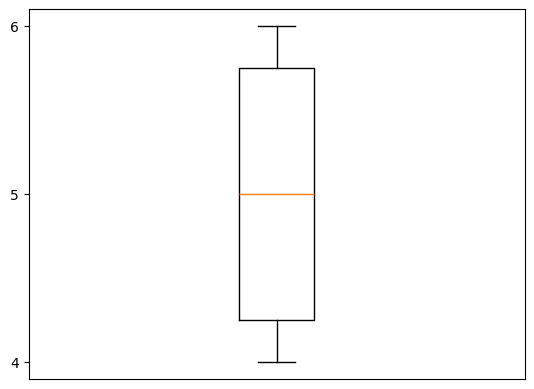
\includegraphics[width=0.5\linewidth]{images/box_plot_simetrico.jpeg}
    \caption{Box plot simétrico}
\end{figure}

\subsubsection{Box plot com dados assimetricos para direita e esquerda}

Vamos considerar os conjuntos de dados

\begin{equation*}
    \text{dados\_assimetricos\_direita} = [2, 3, 3, 4, 3, 2, 3, 4, 10]
\end{equation*}

\begin{equation*}
    \text{dados\_assimetricos\_esquerda} = [10, 9, 8, 9, 10, 8, 9, 2]
\end{equation*}

\begin{figure}[H]
    \centering
    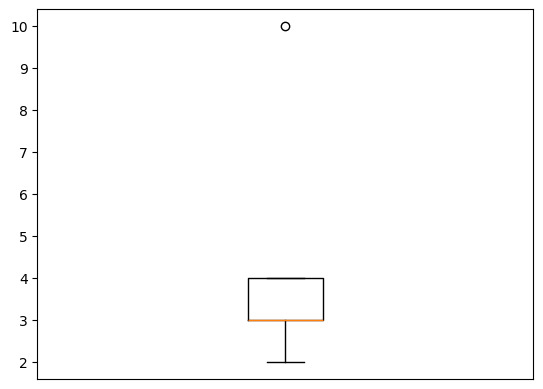
\includegraphics[width=0.5\linewidth]{images/box_plot_assimetrico_direita.jpeg}
    \caption{Box plot assimétrico para direita}
\end{figure}

\begin{figure}[H]
    \centering
    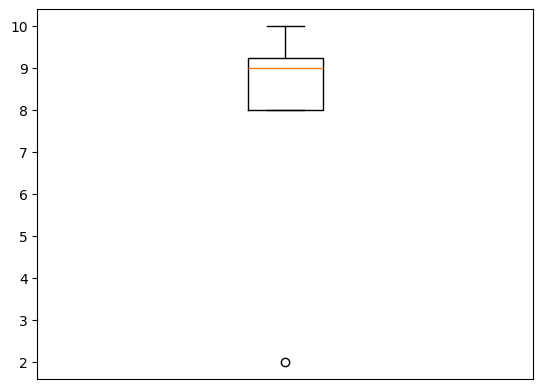
\includegraphics[width=0.5\linewidth]{images/box_plot_assimetrico_esquerda.jpeg}
    \caption{Box plot assimétrico para esquerda}
\end{figure}

\subsection{Quando um valor é considerado outlier?}

Um outlier é um valor atípico, seja em uma situação em que o valor é muito maior do que o padrão ou muito menor. É importante que um outlier seja tratado corretamente durante uma análise de dados pois eles podem: 

\begin{itemize}
    \item Distorcer a média
    \item Aumentar muito o desvio padrão
    \item Indicar anomalias 
    \item Sugerir que a distribuição não é normal
\end{itemize}

\subsubsection{Como identificar outliers utilizando o método IQR}

Um valor é considerado $x_{i}$ é considerado outlier se:

\begin{equation}
    x_{i} < Q1 - 1.5 \times IQR
\end{equation}

ou

\begin{equation}
    x_{i} > Q3 + 1.5 \times IQR
\end{equation}

Em Python:

\begin{pythoncode}
import pandas as pd 

df = pd.read_csv('exemplo.csv')

Q1 = df.quantile(0.25)
Q3 = df.quantile(0.75)

IQR = Q3 - Q1

limite_inferior = Q1 - 1.5 * IQR
limite_superior = Q3 + 1.5 * IQR

outliers = df[(df < limite_inferior) | (df > limite_superior)]

print(outliers)
\end{pythoncode}

\subsubsection{Como identificar outliers utilizando Box plot?}

Em um box plot, os pontos que estiverem acima do bigode supeior e abaixo do bigode inferior são outliers.

\subsubsection{Como identificar outliers utilizadno o método z-score?}

O método \textbf{z-score} identifica outliers medindo \textbf{quantos devios-padrão} um valor está distante da média.

O z-score é definido como:

\begin{equation*}
    z_i = \frac{x_i - \mu}{\sigma}
\end{equation*}

onde: 

\begin{itemize}
    \item $x$ é o valor observado
    \item $\mu$ é a média 
    \item $\sigma$ é o desvio padrão
\end{itemize}

Um valor é considerado outlier se:

\begin{equation}
    |z| > 3
\end{equation}

A ideia vem da regra empírica da distribuição normal:

\begin{itemize}
    \item 68\% dos dados $\rightarrow$ até $1\sigma$
    \item 95\% dos dados $\rightarrow$ até $2\sigma$
    \item 99.7\% dos dados $\rightarrow$ até $3\sigma$
\end{itemize}

Assim, se um dados estiver além da distância $3\sigma$, é considerado raro.

Utilizando Python:

\begin{pythoncode}
import pandas as pd 

df = pd.read_csv('exemplo.csv')

z_scores = (df - df.mean()) / df.std()

outilers = df[abs(z_scores) > 3]

print(outliers)
\end{pythoncode}

\subsection{Como interpretar o coeficiente de relação de Pearson?}

Utilizamos o coeficiente de relação de Pearson para avaliar a correlação entre duas variáveis que possuem relação linear. Para calcular o coeficiente de correlação de Pearson, fazemos:

\begin{equation}
    r = \frac{\displaystyle \sum_{i = 1}^{n}(x_i - \bar{x})(y_i - \bar{y})} {(n - 1)\sigma_x\sigma_y}
\end{equation}

Assim:

\begin{itemize}
    \item se $r = + 1$, as variáveis possuem correlação positiva perfeita. uma variável sempre vai ter correlação positiva perfeita consigo, vide desigualdade de Cauchy-Schwarz;
    \item se $r = - 1$, as variáveis possuem correlação negativa perfeita (inversamente proporcionais, quando uma está no seu máximo a outra está no seu mínimo);
    \item se $r = 0$, as variáveis não possuem correlação (ao menos não linear).
\end{itemize}

Utilizando Python, podemos plotar um Heatmap mostrando a relação entre as variáveis:

\begin{pythoncode}
import matplotlib.pyplot as plt
import numpy as np

corr = df.corr()

plt.figure()
plt.imgshow(corr)
plt.colorbar()

plt.show()
\end{pythoncode}

\subsubsection{Como provar que o coeficiente de Pearson sempre está entre -1 e +1?}

Na forma vetoria, podemos escrever:

\begin{align*}
    &\tilde{x}_{i} = x_i - \bar{x} \\
    &\tilde{y}_{i} = y_i - \bar{y}
\end{align*}

com

\begin{equation*}
    \tilde{x} = (\tilde{x}_1, ..., \tilde{x}_n), \ \tilde{y} = (\tilde{y}_1, ..., \tilde{y}_n)
\end{equation*}

podemos então reescrever o coeficiente de relação de pearson como sendo:

\begin{equation*}
    r = \frac{\tilde{x}\cdot \tilde{y}}{|\tilde{x}||\tilde{y}|}
\end{equation*}

Da desigualdade de Cauchy-Schwarz:

\begin{equation*}
    |\tilde{x} \cdot \tilde{y}| \leq |x||y|
\end{equation*}

que pode ser reescrita como

\begin{equation*}
    \frac{|\tilde{x}\cdot \tilde{y}|}{|\tilde{x}||\tilde{y}|} \leq 1
\end{equation*}

como o lado esquerdo é o próprio r:

\begin{equation*}
    r \leq 1
\end{equation*}

\subsection{Como explorar duas ou mais variáveis com gráficos de dispersão?}

Os gráficos de dispersão são amplamente utilizados na análise multivariada para investigar a relação entre duas variáveis quantitativas. Eles permitem identificar padrões, tendências, correlações e possíveis outliers de forma visual e intuitiva.

No entanto, são mais indicados para conjuntos de dados pequenos ou amostras. Em bases muito grandes, a sobreposição excessiva de pontos pode tornar o gráfico poluído e de difícil interpretação (overplotting).

Uma alternativa é a \textbf{compartimentação hexagonal}. Nesse método, em vez de representar cada observação individualmente, o plano cartersiano é dividido em células hexagonais. Os registros são agrupados dentro de cada hexágono e a cor indicaa quantidade de observações naquele compartimento.

Em Python:

\begin{pythoncode}
ax = df.hexbin(x='Coluna_do_eixo_x', y='Coluna_do_eixo_y', gridsize=Tamanho_do_grid)

plt.show()
\end{pythoncode}

\section{Amostragem}

\subsection{Viés de amostragem}

Um viés de amostragem ocorre quando a amostra analisada não representa adequadamente a população de interesse, em razão do modo como foi selecionada. Nesse caso, a distorção não é aleatória, mas sistemática: determinados indivíduos têm mais probabilidade de compor a amostra. Como resultado, as conclusões obtidas podem diferir significativamente da realidade e esse erro tende a se repetir sempre que o mesmo método de coleta é utilizado.

Um exemplo pode ser observado nas avalições de companhias aéreas em sites especializados. Os passageiros normalmente registram sua opinião após experiências muito negativas (como atrasos longos, extravio de bagagem ou mau atendimento) ou, menos frequentemente, após experiências excepcionalmente positivas. Enquanto isso, aqueles que tiveram um voo dentro do esperado tendem a não se manifestar. Assim, as avaliações disponíveis podem super-representar situações extremas e não refletir a experiência típica da maioria dos passageiros.

\subsection{Viés de seleção}

O viés de seleção ocorr  quando os dados utilizados em uma análise não são escolhidos de forma independente do resultado que se deseja avaliar, produzindo estimativas sistematicamente distorcidas.

No contexto de Machine Learning, é comum fixarmos um seed para tornar reprodutível a divisão entre treino e teste. Cada escolha de seed gera uma participação diferente dos dados e, portanto, uma estimativa distinta da performance do modelo.

Se testarmos várias seed e selecionarmos aquela que produz o melhor resultado, estaremos escolhendo o máximo (ou mínimo) de um conjunto de variáveis aleatórias. Seja

\begin{equation*}
    \hat{R}_1, \hat{R}_2, ..., \hat{R}_k
\end{equation*}

as estimativas de erro obtidas com $k$ participações diferentes. Ao selecionar

\begin{equation*}
    \hat{R}_{favoravel} = \min_i \hat{R}_i
\end{equation*}

introduzimos um viés otimista, pois

\begin{equation*}
    \mathcal{E}[\min(\hat{R_1},..., \hat{R}_k)] \leq \mathcal{E}[\hat{R}_i]
\end{equation*}

Ou seja, o melhor resultado observado tende, em média, a subestimar o erro real do modelo.

\subsection{Teorema de limite central}

O teorema de limite central diz que as médias extraídas de múltiplas amostras serão semelhantes à uma distribuição normal, mesmo se a população fonte não é normalmente distribuída, contanto que o tamanho da amostra seja grande o bastante e o desvio dos dados da normalidade não seja muito grande.

\subsubsection{Prova do teorema de limite central}

Para variáveis aleatórias i.i.d

\begin{equation*}
    X_1, X_2, ...
\end{equation*}

com:

\begin{itemize}
    \item média $\mu$
    \item variância $\sigma^2 < \infty$
\end{itemize}

queremos provar que 

\begin{equation*}
    \frac{\sqrt{n}}{\sigma}(\bar{X}_n - \mu) \rightarrow \mathcal{N}(0, 1)
\end{equation*}

A soma das variáveis aleatórias tem:

\begin{align*}
    &E(X_1, X_2, ..., X_{n - 1}, X_n) = n\mu \\
    &Var(X_1, X_2, ..., X_{n - 1}, X_n) = n\sigma^2 
\end{align*}

Normalizamos como:

\begin{equation*}
    Z_n = \frac{X_1 + ... + X_n - n\mu}{\sqrt{n\sigma^2}} = \displaystyle \sum_{i = 1}^{n}\frac{X_i - \mu}{\sqrt{n\sigma^2}}
\end{equation*}

onde definimos

\begin{equation*}
    Y_i = \frac{X_i - \mu}{\sigma}
\end{equation*}

com

\begin{align*}
    &E(Y_i) = 0 \\
    &Var(Y_i) = 0
\end{align*}

Logo:

\begin{equation*}
    Z_n = \sum_{i = 1}^{n}\frac{1}{\sqrt{n}}Y_i
\end{equation*}

Aplicando a função característica em $Z_n$:

\begin{equation*}
    \varphi Z_n(t) = \prod_{i = 1}^{n}\varphi Y_i\left(\frac{t}{\sqrt{n}}\right) = \left[\varphi Y_i\left( \frac{t}{\sqrt{n}}\right)\right]^n
\end{equation*}

Utilizando expansão de Taylor:

\begin{equation*}
    \varphi Y_i\left(\frac{t}{\sqrt{n}}\right) = 1 - \frac{t^2}{2n} + \mathcal{o}\left(\frac{t^2}{n}\right), \  \left(\frac{t}{\sqrt{n}}\right) \rightarrow 0
\end{equation*}

Assim

\begin{equation*}
    \varphi Z_n(t) = \left(1 - \frac{t^2}{2n} + \mathcal{o}\left(\frac{t^2}{n}\right)\right)^n \rightarrow e^{-\frac{-1}{2}t^2}, \ n \rightarrow \infty
\end{equation*}

A função característica da normal padrão é:

\begin{equation*}
    \varphi(t) = e^{-\frac{1}{2}t^2}
\end{equation*}

Então

\begin{equation*}
    Z_n \xrightarrow[]{d} \mathcal{N}(0, 1)
\end{equation*}

\subsection{Bootstrap}

O bootstrap é uma técnica de reamostragem que consiste em gerar múltiplas amostras a partir de um conjunto de dados original, selecionando observações aleatoriamente com reposição. Cada amostra bootstrap possui o mesmo tamanho da amostra original, mas pode conter observações repetidas e omitir outras.

Ao repetir um processo muitas vezes, obtemos uma distribuição empírica da estatística de interesse (como média, mediana, coeficientes de um modelo ou métricas de desempenho). Essa distribuição permite estimar o erro padrão, intervalos de confianças e víes do estimador, sem depender de suposições fortes sobre a distribuição dos dados.

O algoritmo para uma reamostragem bootstrap da média para uma amostra de tamanho n é:

\begin{enumerate}
    \item Extraia um valor de amostra, registre e reponha;
    \item Repita n vezes;
    \item Registre a média dos n valores reamostrados;
    \item Repita o passo 1 e 3 R vezes;
    \item Use os R resultados para: calcular seu desvio-padrão (isso estima o erro-padrão da média da amostra), produzir um histograma ou um gráfico de caixas e encontrar um intervalo de confiança.
\end{enumerate}

O número R de iterações do bootstrap é definido de forma arbitrárias, quanto mais iterações são feitas, mais precisa é a estimativa do erro-padrão ou intervalo de confiança.

Em Python, podemos utilizar o método \textbf{resample}, da biblioteca \textbf{scikit-learn}:

\begin{pythoncode}
results = []

for nrepeat in range(1000):
    sample = resample(loans_income)
    results.append(sample.median())

results = pd.Series(results)
print('Bootstrap Statistics:')
print(f'original: {loans_income.median()}')
print(f'bias: {results.mean() - loans_income.median()}')
print(f'std.error: {results.std()}')
\end{pythoncode}

\subsubsection{O que é bagging?}

Bagging é uma técnica de amostragem que melhora a estabilidade de modelos de machine learning reduzindo a variância. A intuição matemática é que se temos estimadores independentes:

\begin{equation*}
    Var\left(\frac{1}{B} \sum_{b =1}^{B} f_b(x)\right) = \frac{1}{B^2}\sum Var(f_b(x))
\end{equation*}

Assim, o passo a passo é:

\begin{enumerate}
    \item Criar amostras bootstrap: gerar várias amostras com reposição, cada uma com tamanho n
    \item Treinar modelos separados: treinamos um modelo em cada amostra. Por exemplo: treinamos n árvores de decisão, cada uma treinada em um bootstrap diferente
    \item Agregamos previsões
\end{enumerate}

\section{Distribuições}

\subsection{Distribuição normal (distribuição gaussiana)}

A distribuição normal é um modelo probabilístico contínuo que descreve fenômenos cuja maioria dos valores se concentra ao redor da média, com simetria perfeita.

A função densidade é 

\begin{equation}
    f(x) = \frac{1}{\sigma \sqrt{2\pi}}exp\left(-\frac{(x - \mu)^2}{2\sigma^2} \right)
\end{equation}

Por conter simetria perfeita:

\begin{itemize}
    \item média = mediana = moda
    \item 68\% dos dados estão em $\mu \pm \sigma$
    \item 95\% dos dados estão em $\mu \pm 2\sigma$
    \item 99.7\% dos dados estão em $\mu \pm 3\sigma$
\end{itemize}

\begin{figure}[H]
    \centering
    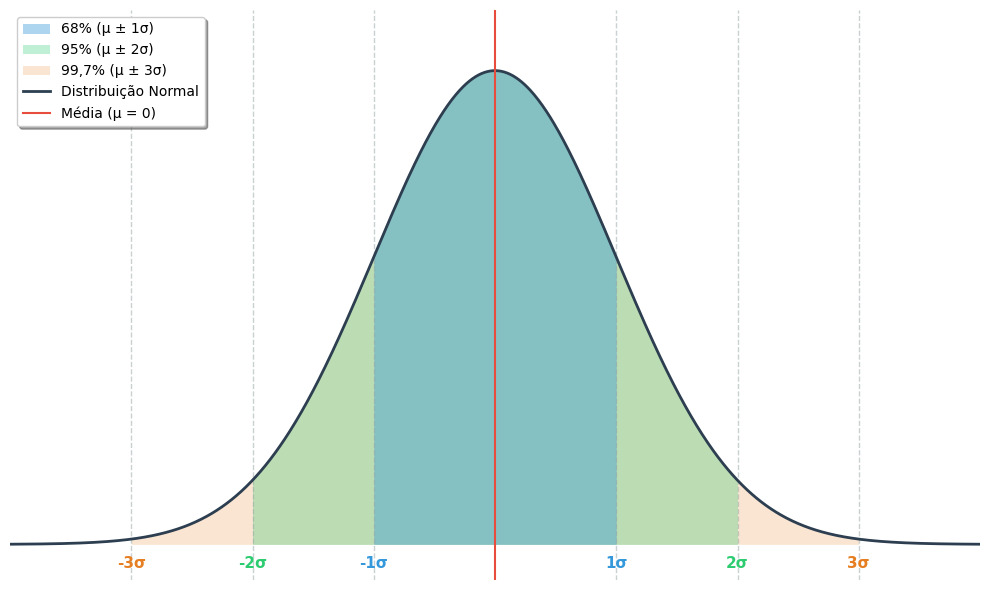
\includegraphics[width=1.0\linewidth]{images/distribuicao_gaussiana.jpeg}
\end{figure}

\subsection{Distribuicao t de Student}

A \textbf{distribuição t de Student} é semelhante à distribuição normal, porém apresenta \textbf{caudas mais espessas}, o que significa maior probabilidade de valores extremos. Essa característica reflete a incerteza adicional introduzida quando o desvio padrão populacional é desconhecido e precisa ser estimado a partir da amostra.

A distribuição t não é única, mas sim uma família de distribuições, que variam de acordo com os graus de liberdade. Quanto maior o tamanho da amostra, maiores são os graus de liberdade e mais a distribuição t se aproxima da distribuição normal. 

A utilização da distribuição t para modelar o comportamento de uma estatística amostral (como a média) pressupõe que essa estatística tenha distribuição aproximadamente normal, fato que pode ser satisfeito pelo teorema do limite central.

A funcao de densidade de probabilidade é dada por:

\begin{equation}
    f(t) = \frac{\Gamma\left(\frac{v + 1}{2}\right)}{\sqrt{\pi v}\Gamma\left(\frac{v}{2}\right)}\left(1 + \frac{t^2}{v}\right)^{-\left(\frac{v + 1}{2}\right)}
\end{equation}

onde $v$ é o número de graus de liberdade.


\subsubsection{O que acontece quando o número de graus de liberdade tende ao infinito?}

Vamos dividir a expressão de $f(t)$ em duas partes:

\begin{equation*}
    f(t) = \underbrace{\frac{\Gamma\left(\frac{v + 1}{2}\right)}{\sqrt{\pi v}\Gamma\left(\frac{v}{2}\right)}}_{ =A}\underbrace{\left(1 + \frac{t^2}{v}\right)^{-\left(\frac{v + 1}{2}\right)}}_{= B}
\end{equation*}

Primeiro, vamos avaliar a parte $A$:

\begin{equation*}
    A = \frac{\Gamma \left(\frac{v + 1}{2}\right)}{\sqrt{\pi v}\Gamma\left(\frac{v}{2}\right)}
\end{equation*}

Usando a aproximação de Stirling para a função Gamma:

\begin{equation*}
    \Gamma(z) \sim \sqrt{2\pi}z^{z - \frac{1}{2}}e^{-z}, \ \text{quando} \ z \rightarrow \infty
\end{equation*}

Aplicando na razão $A$:

\begin{equation*}
    \frac{\Gamma\left(\frac{v + 1}{2}\right)}{\Gamma \left(\frac{v}{2}\right)} \sim \left(\frac{v}{2}\right)^{1/2}
\end{equation*}

Então:

\begin{equation*}
    A \sim \frac{\sqrt{v/2}}{\sqrt{\pi v}} = \frac{1}{\sqrt{2\pi}}
\end{equation*}

Agora, vamos avaliar a parte exponencial $B$:

\begin{equation*}
    B = \left(1 + \frac{t^2}{v}\right) = exp\left[-\frac{v + 1}{2}\ln \left(1 + \frac{t^2}{v}\right)\right]
\end{equation*}

Quando $v \rightarrow \infty$, temos que $\frac{t^2}{v} \rightarrow 0$. Assim, utilizando expansão de Taylor:

\begin{equation*}
    \ln\left(1 + \frac{t^2}{v}\right) \approx \frac{t^2}{v}
\end{equation*}

substituindo:

\begin{equation*}
    B \approx exp \left[- \frac{v + 1}{2} \cdot \frac{t^2}{v}\right] = exp \left[- \frac{t^2}{2} \cdot \frac{v + 1}{v}\right] = exp \left[-\frac{t^2}{2}\right]
\end{equation*} 

Então:

\begin{equation*}
    \lim_{v \rightarrow \infty} f(t) = \lim_{v \rightarrow \infty} \frac{\Gamma\left(\frac{v + 1}{2}\right)}{\sqrt{\pi v}\Gamma\left(\frac{v}{2}\right)}\left(1 + \frac{t^2}{v}\right)^{-\left(\frac{v + 1}{2}\right)} = \frac{1}{\sqrt{2\pi}}e^{-\frac{t^2}{2}} = \mathcal{N}(0, 1)
\end{equation*}

\begin{figure}[H]
    \centering
    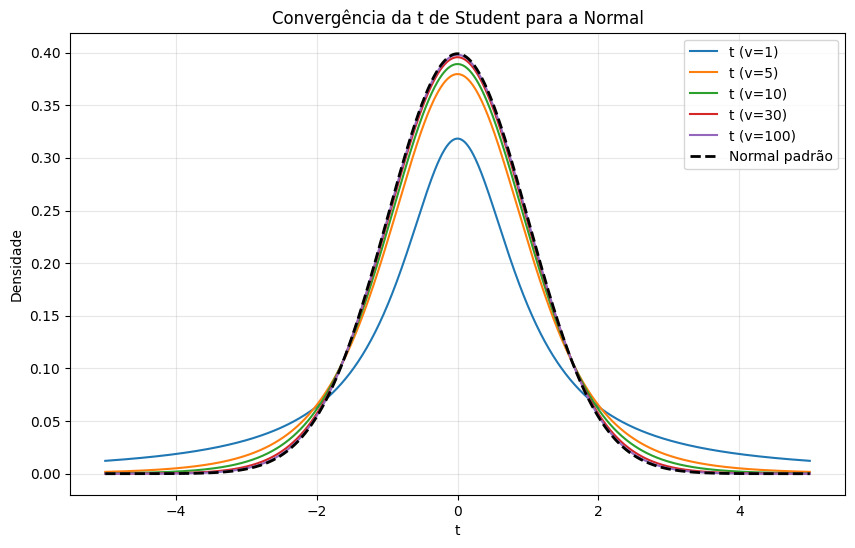
\includegraphics[width=1.0\linewidth]{images/student_e_normal.jpeg}
\end{figure}

\subsubsection{Gráfico QQ}

O gráfico QQ é uma ferramenta gráfica utilizada para comparar duas distribuições de probabilidade, plotando seus quantis um contra o outro. Ele é usado para responder à pergunta: "meus dados se comportam como a distribuição que estou assumindo?"

\begin{itemize}
    \item \textbf{Eixo y}: os z-scores dos dados (seus valores transforamdos para terem média 0 e desvio padrão 1)
    \item \textbf{Eixo x}: os quantis teóricos da distribuição normal padrão (que são os z-scores esperados)
\end{itemize}

Para construção:

\vspace{0.25cm}

\textbf{Passo 1: calcular os z-scores dos dados} 

\begin{equation*}
    Z_{observado} = \frac{x - \bar{x}}{s}
\end{equation*}

onde 

\begin{itemize}
    \item $x$ é o valor original 
    \item $\bar{x}$ é a média dos dados 
    \item $s$ é o desvio padrão dos dados 
\end{itemize}

Se as duas distribuições sendo comparadas são semelhantes, os pontos no gráfico QQ vão cair aproximadamente ao longo de uma linha reta (geralmente a linha $y = x$, ou a linha de regressão dos pontos).

\vspace{0.25cm}

\textbf{Passo 2: ordenar os z-scores}

Colocamos os z-scores calculados em ordem crescente.

\vspace{0.25cm}

\textbf{Passo 3: calcular os quantis teóricos}

Para cada posição dos dados ordenados, calculamos qual seria o z-score esperado em uma distribuição normal perfeita.

\vspace{0.25cm}

\textbf{Passo 4: plotar}

Cada ponto no gráfico de dispersão é um par, com a cordenada x o z-score teórico (quantil normal esperado) e a coordeanda y o z-score observado (dado padronizado).

Podemos gerar uma figura de um gráfico QQ para uma amostra de valores aleatoriamente gerados de uma distribuição normal. Como os valores são amostras da própria distribuição normal, eles devem seguir a reta $y = x$. Para isso:

\begin{pythoncode}
import numpy as np
import scipy.stats as stats
import matplotlib.pyplot as plt

fig, ax = plt.subplots(figsize=(8,6))
norm_sample = stats.norm.rvs(size=1000)

stats.probplot(norm_sample, plot=ax)
plt.tight_layout()
plt.show()
\end{pythoncode}

\begin{figure}[H]
    \centering
    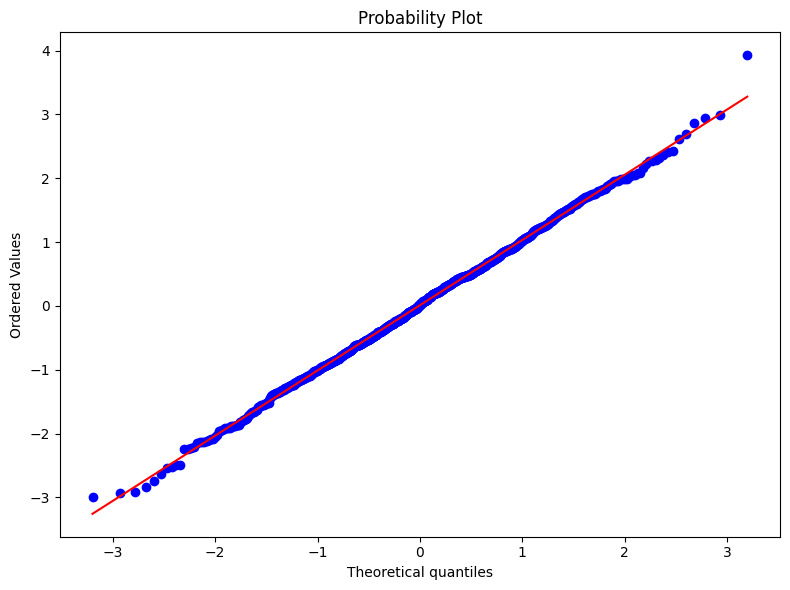
\includegraphics[width=0.85\linewidth]{images/grafico_QQ_distribuicao_normal_padrao.jpeg}
\end{figure}

\section{Experimentos estatísticos}

\subsection{Teste de hipótese}

Um teste de hipótese (ou teste de significância) é uma ferramenta estatística inferencial utilizada para avaliar se um efeito observado nos dados pode ser atribuído ao acaso ou se há evidências suficientes para considerar que ele reflete um fenômeno real na população.

Assim, o teste de hipótese ajuda a decidir entre duas explicações possíveis:

\begin{enumerate}
    \item o resultado ocorreu devido à variabilidade aleatória natural dos dados;
    \item  o resultado é estatisticamente significativo e dificilmente seria observado apenas pelo acaso.
\end{enumerate}

Para isso:

\begin{itemize}
    \item Hipótese nula ($H_0$): é a afirmação inicial assumida como verdadeira até que haja evidências contrárias. Geralmente representa a ausência de efeito, diferença ou associação.
    \item Hipótese alternativa ($H_1$): é a afirmação que contradiz a hipótese nula. Representa a presença de efeito, diferença ou associação.
\end{itemize}

\subsection{Reamostragem}

A Reamostragem consiste em amostrar repetidamente a partir dos dados observados com o objetivo de avaliar a variabilidade aleatória de uma estatística. Para isso, podemos utilizar o processo \textit{bootstrap} e \textit{testes de permutação}. O \textit{bootstrap} é utilizado para avaliar a confiabilidade de uma estimativa, enquanto os testes de permutação são usados para testar hipóteses, geralmente envolvendo dois ou mais grupos.

\subsubsection{Teste de permutação aleatória}

No teste de permutação, queremos provar a hipótese nula de que os tratamentos aos quais os grupos foram expostos não produzem diferença sistemática na variável de interesse. Sob hipótese nula, as observações são provenientes da mesma distribuição e as etiquetas do grupos são irrelevantes. Para executar o teste de permutação:

\begin{enumerate}
    \item Combinar os resultados dos diferentes grupos em um único conjuto de dados.
    \item Embaralhar os dados combinados.
    \item Divdir os dados embaralhados em dois grupos, preservando o tamanho dos grupos originais.
    \item Calcular a estimativa de interesse (por exemplo, diferença de médias) para a nova configuração.
    \item Repetir os passos K vezes para  construir a distribuição de permutação da estatística desejada.
\end{enumerate}

A comparação entre a estatística observada e a distribuição de permutação permite calcular o \textit{p-valor}. Se a diferença observada estiver situada em uma região central da distribuição permutada, concluímos que o resultado é compatível com a variabilidade aleatória esperada sob a hipótese nula. Se a diferença observada estiver localizada nas caudas da distribuição de permutação, isso indica que tal resultado seria improvável de ocorrer apenas pelo acaso, fornecendo evidência contra a hipótese nula.

\subsection{Nível de significância \texorpdfstring{$\alpha$}{α}}

O nível de significância $\alpha$ é a probabilidade máxima que você aceita cometer um erro tipo I. Em geral, é escolhido $\alpha = 0.05$, o que equivale dizer que aceitamos o risco de 5\% de cometer um erro do tipo I.

\subsection{Significância estatística}

Um resultado é considerado estatisticamente significativo quando seria improvável de ocorrer caso a hipótese nula fosse verdadeira. Dizemos que um resultado é estatisticamente significado quando o p-valor associado ao teste é menor que um nível de significância previamente estabelecido ($\alpha$).

\subsection{p-valor}

Dado um modelo que representa a hipótese nula, o p-valor é a probabilidade de observar uma estatística de teste tão extrema quanto, ou mais extrema que, aquela obtida nos dados, assumindo que a hipótese nula seja verdadeira. 

Formalmente, se $T$ é a estatística de teste e $t_{obs}$ é o valor observado, o p-valor é dado por:

\begin{equation}
    p = P(T \ge t_{obs} \mid H_0)
\end{equation}

\begin{enumerate}
    \item Se $p \leq \alpha \rightarrow$ rejeito $H_0$
    \item Se $p > alpha \rightarrow$ não rejeito $H_0$
\end{enumerate}

\subsection{Erro do Tipo I \texorpdfstring{($\alpha$)}{(α)}}

O erro do tipo I acontece quando rejeitamos a hipótese nula quando ela é verdadeira. A probabilidade de cometer esse erro é definida previamente pelo \textbf{nível de significância ($\alpha$)}. 

Por exemplo, ao realizar um teste A/B com o objetivo de aumentar a taxa de conversão de leas, formulamos a hipótese nula, como a afirmação de que a nova implementação não altera a taxa de conversão em relação à versão original.

Se, com base nos resultados do teste, rejeitarmos essa hipótese e concluirmos que a nova versão melhora a conversão quando, na verdade, a diferença observada foi apenas fruto da variabilidade aleatória, estaremos cometendo um erro do tipo I (um falso positivo).

\subsection{Erro do Tipo II \texorpdfstring{($\beta$)}{β}}

O erro do tipo II ocorre quando aceitamos a hipótese nula mesmo ela sendo falsa. 

A probabilidade de cometer esse erro é representada por $\beta$, e está diretamente realcionada ao poder estatístico do teste, definido por $1 - \beta$, que mede a capacidade de identificar um efeito real quando ele de fato está presente.

No contexto de um teste A/B para aumentar a taxa de conversão de leads, a hipótese nula afirma que a nova implementação não altera a taxa de conversão. Suponha, porém, que a nova versão realmente aumente a conversão.

Se, ao final do experimento, não rejeitarmos a hipótese nula (concluindo que não há diferença significativa), estaremos cometendo um erro do tipo II (falso negativo). Nesse caso, uma melhoria real deixaria de ser implementada por falta de evidência estatística suficiente.

\subsection{ANOVA}

Suponha que, em vez de um teste A/B, desejemos comparar quatro grupos (A/B/C/D), cada um contendo observações numéricas. O procedimento estatístico utilizado para verificar se existe diferença estatisticamente significativa entre as médias de múltiplos grupos é chamado de ANOVA.

A ideia da ANOVA é comparar a variabilidade entre os grupos com a variabilidade dentro dos grupos. Se a variabilidade entre as médias for grande o suficiente em relação à variabilidade interna, temos evidência contra a hipótese nula de que todas as médias são iguais. 

\begin{enumerate}
    \item Reúna todas as observações dos quatro grupos em um único conjunto;
    \item Embaralhe os valores aleatoriamente;
    \item Divida-os em quatro grupos com o mesmo tamanho original (por exemplo, cinco observações por grupo);
    \item Calcule a média de cada grupo reamostrado;
    \item Calcule a variância entre as médias desses quatro grupos;
    \item Repita os passos 2 a 5 K vezes.
\end{enumerate}

Ao final, compare a variância observada nos dados reais com as variâncias obtidas nas reamostragens. A proporção de vezes que a variância reamostrada é maior ou igual à variância observada corresponde ao p-valor. Se essa proporção for pequena (menor que $\alpha$), isso indica que a diferença observada entre as médias dificilmente teria ocorrido apenas por aleatoriedade, fornecendo evidência contra a hipótese nula de igualdade das médias.

\subsection{Consideração quanto a modelos preditivos}

Para a modelagem preditiva, o risco de obter um modelo ilusório cuja eficácia aparente é mais um produto do acaso é mitigado pela validação cruzada e pelo uso de uma amostra de validação.


\subsubsection{Exemplo}

Por exemplo, em um site de e-commerce, podemos avaliar se uma alteração na interface (UI/UX) aumenta a taxa de conversão de leads em comparação com a versão original. Para isso, realizamos um \textbf{teste A/B}, no qual os usuários são dividios aleatoriamente em dois grupos: o grupo A (tratamento), que recebe a nova versão da UI/UX e o grupo b (controle), que permanece com a versão original. A formulação das hipóteses é feita da seguinte forma:

\begin{itemize}
    \item $H_0$: a nova UI/UX não altera a taxa de conversão. Ou seja, a taxa de conversão do grupo A é igual à do grupo B.
    \item $H_1$: a nova UI/UX aumenta a taxa de conversão. Ou seja, a taxa de conversão do grupo A é maior que a do grupo B.
\end{itemize}

Matematicamente, se $p_A$ representa a taxa de conversão da nova versão e $p_B$ a taxa de versão original, temos:

\begin{align*}
    &H_0: p_A = p_B \\
    &H_1: p_A > p_B
\end{align*}

\subsection{Algoritmo do bandido multibraços (Multi-Armed Bandit - MAB)}

O algoritmo do bandido multibraçõs (Multi-Armed Bandit) é uma abordagem para experimentação
online que busca equilibrar exploração (testar alternativas) e exploração do melhor resultado
(exploit). Diferentemente do teste A/B tradicional (que mantém proporções fixas e alocação durante
todo o experimento), o MAB permite otimização explícita ao longo do tempo, direcionando progressivamente
mais usuários para a alternativa que apresenta melhor desempenho. Isso possibilita uma tomada
de decisão potencialmente mais rápida e com menor perda de oportunidade.

Um dos algoritmos mais simples dessa família é o $\varepsilon$-greedy. Para um teste A/B,
seu funcionamento pode ser descrito da seguinte forma:

\begin{enumerate}
\item Gere um número aleatório com distribuição uniforme no intervalo entre 0 e 1.
\item Se o número estiver no intervalo entre 0 e $\varepsilon$ (onde $\varepsilon \in [0,1]$, geralmente pequeno), execute uma etapa de exploração:
\begin{itemize}
\item Escolha aleatoriamente entre as ofertas A e B (por exemplo, com probabilidade 50/50).
\end{itemize}
\item Se o número for maior ou igual a $\varepsilon$, execute a etapa de exploração do melhor resultado (exploit):
\begin{itemize}
\item Mostre a oferta que apresenta a maior taxa de resposta estimada até o momento.
\end{itemize}
\end{enumerate}

$\varepsilon$ é um único parâmetro que controle esse algoritmo. Se épsilon é 1, temos um 
experimento A/B padrão simples (alocação aleatória entre A e B para cada indivíduo). 
Se épsilon é 0, temos um algoritmo puramente greedy (um que escolhe a melhor opção 
imediata disponível).

\subsection{Tamanho da amostra}

Para definirmos o tamanho da amostra necessária para avaliar um teste A/B, precisamos 
definir:

\begin{itemize}
    \item Tamanho do efeito que queremos detectar;
    \item Nível de significância ($\alpha$) em que o teste será realizado;
    \item Potência do teste ($1 - \beta$)
\end{itemize}

O tamanho do efeito que queremos detectar é a melhoria mínima que queremos encontrar.
Por exemplo, podemos definir que o experimento só vale a pena se houver um aumento de 
pelo menos 2 pontos percentuais na taxa de conversão (de 10\% para 12\%).

O nível de significância ($\alpha$) é a probabilidade de cometer um erro do Tipo I, ou seja,
rejeitar a hipótese nula quando ela é verdadeira. 

A potência do teste é a probabilidade de detectar o efeito definido caso ele realmente exista 
(encontrar uma diferença real).

Em Python, podemos calcular o tamanho da amostra fazendo:

\begin{pythoncode}
from statsmodels.stats.power import NormalIndPower
from statsmodels.stats.proportion import proportion_effectsize 

# taxas esperadas
p1 = 0.10 # taxa atual de conversao (1\%)
p2 = 0.12 # nova meta de conversao (12\%)

effect_size = proportion_effectsize(p1, p2)

alpha = 0.05
power = 0.8

analysis = NormalIndPower()

n = analysis.solve_power(
    effect_size=effect_size,
    alpha=alpha,
    power=power,
    alternative='two-sided'
)

print(f"Tamanho da amostra por grupo: {round(n)}")
\end{pythoncode}

\section{Predição}

\subsection{Regressão linear simples}

A regressão linear simples é um método estatístico utilizado para modelar 
a relação entre uma variável $Y$ e uma única variável explicativa $X$.

Seu objetivo é estimar quanto, em média, $Y$ varia quando $X$ aumenta
em uma unidade, assumindo que essa relação possa se aproximar de algo linear.

O modelo é representado por:

\begin{equation}
    Y = b_0 + b_1 X
\end{equation}

\begin{itemize}
\item $b_0$ é o intercepto, isto é, o valor esperado de $Y$ quando $X = 0$;
\item $b_1$ é o coeficiente angular (inclinação da reta), que representa a variação média em $Y$ para cada aumento unitário em $X$;
\item $Y$ é a variável resposta (target);
\item $X$ é a variável preditora (feature).
\end{itemize}

Em Python, podemos ver o quão os dados se ajustam a uma reta fazendo:

\begin{pythoncode}
from sklearn.linear_model import LinearRegression

predictors = ['Coluna_exemplo']
outcome = 'Exemplo'

model = LinearRegression()
model.fit(lung[predictors], lung[outcome])

print(f'Intercepto: {model.intercept_:.3f}')
print(f'Coeficiente: {model.coef_[0]:.3f}')
\end{pythoncode}

Em geral, os dados não se adequam perfeitamente à reta estimada, então
na equação de regressão utilizamos um termo $e_i$ para representar a variação
não explicada pelo modelo:

\begin{equation}
    Y_i = b_0 + b_1X_i + e_i
\end{equation}

Após estimar os coeficientes $\hat{b}_0$ e $\hat{b}_1$, podemos calcular os 
valores ajustados (ou preditos) pela reta:

\begin{equation}
    \hat{Y}_i = \hat{b}_0 - \hat{b}_1X_i
\end{equation}

O resíduo de cada observação é a diferença etnre o valor observado e o valor ajustado:

\begin{equation}
    \hat{e}_i = Y_i - \hat{Y}_i
\end{equation}

Em Python, podemos obter os valores \textit{ftted} e os valores residuals:

\begin{pythoncode}
# valores ajustados (previsoes do modelo)
fitted = model.predict(lung[predictors])

# residuos (diferenca entre valores observados e ajustados)
residuals = lung[outcome] - fitted
\end{pythoncode}

A melhor reta escolhida pelo modelo é aquela que minimiza a soma residual dos quadrados:

\begin{equation}
    RSS(b_0, b_1) = \sum_{i = 1}^{n}(Y_i - Y_i)^2 = \sum_{i = 1}^{n}(Y_i - b_0 - b_1X_i)^2
\end{equation}

Para encontrarmos os $\hat{b}_0$ e $\hat{b}_1$ que otimizam $RSS(b_0, b_1)$:

\begin{align*}
    &\frac{\partial}{\partial b_0}RSS(b_0, b_1) = -2\sum_{i = 1}^{n}(Y_i - b_0 - b_1X_i) = 0 \\
    &\frac{\partial}{\partial b_1}RSS(b_0, b_1) = -2\sum_{i = 1}^{n}(Y_i - b_0 - b_1X_i) = 0
\end{align*}

A solução explícita da equação retorna

\begin{align*}
    &\hat{b}_1 = \frac{\sum(X_i - \bar{X})(Y_i - \bar{Y})}{\sum(X_i - \bar{X})^2} = \frac{Cov(X, Y)}{Var(X)} \\
    &\hat{b}_0 = \bar{Y} - \hat{b}_1\bar{X}
\end{align*}

\subsection{Regressão linear múltipla}

A regressão linear múltipla é utilizada quando existe duas ou mais variáveis preditoras:

\begin{equation}
    Y = b_0 + b_1X_1 + \sum_{i = 2}^{n}b_iX_i
\end{equation}

Aqui, precisamos tomar cuidado: adicionar mais variáveis ao modelo não quer dizer que vamos ter resultados melhores.
É preciso analisar como os dados se relacionam com a variável analisada bem como se ela já não é descrita por outra.
Incluir variáveis adicionais reduz o RMSE e aumenta o $R^2$ para os dados de treinamento, logo, esses não são 
indicados para guiar a escolha do modelo. Para encontrar o modelo ideal (isto é, com a quantidade e variáveis ideiais),
podemos incluir e excluir sucessivamente as variáveis preditoras para encontrar um modelo que aprimora o $R^2$ ajustado.

Para isso:

\begin{itemize}
    \item Definimos uma função que retorna um modelo ajustado para determinado conjunto de variáveis;
    \item Definimos uma função que retorna um score para determinado modelo e conjunto de variáveis.
\end{itemize}

Em Python, podemos fazer da seguinte forma:

\begin{pythoncode}
from sklearn.linear_model import LinearRegression

def train_model(variables):
    if len(variables) == 0:
        return None 
    model = LinearRegression()
    model.fit(X[variables], y)
    return model 

def score_model(model, variables):
    n = len(y)
    p = len(variables)
    if len(variables) == 0:
        return 0 
    r2 = model.score(X[variables], y) 
    r2_adj = 1 - (1 - r2) * (n - 1) / (n - p - 1)
    return r2_adj

best_model, best_variables = stepwise_selection(X.columns, train_model, score_model, verbose=True)

print(f'Intercept: {best_model.intercept_:.3f}')
print('Coeficientes:')
for name, coef in zip(best_variables, best_model.coef_):
    print(f' {name}: {coef}')
\end{pythoncode}

\subsection{Regressão ponderada}

A regressão ponderada (Weighted Least Squares - WLS) é uma variação 
da regressão linear tradicional na qual atribuímos pesos diferentes 
às observações do conjunto de dados. O objetivo é dar maior importância 
às observações consideradas mais confiáveis ou mais relevantes para 
o problema em análise. Aqui, minimizamos:

\begin{equation}
    \sum_{i = 1}^{n} \omega_i (y_i - \hat{y}_i)^2
\end{equation}

em que $\omega_i$ representa o peso associado à $i$-ésima observação. 

Por exemplo, em um conjunto de dados de valores imobiliários, registros 
antigos podem ser menos representativos das condições atuais do mercado.
Nesse caso, podemos atribuir pesos menores às observações mais antigas 
e pesos maiores às mais recentes, fazendo com que o modelo ajuste a reta 
priorizando dados mais atuais.

No \textit{scikit-learn}, essa ponderação pode ser implementada passando 
o argumento \texttt{sample\_weight} ao método \texttt{fit}, permitindo que 
cada observação contribua de forma diferenciada para o ajuste do modelo.

\subsection{Variáveis fatoriais na regressão}

As variáveis fatoriais (ou variáveis categóricas) representam características qualitativas,
como cor, cidade, tipo de produto ou nível educacional. Diferentemente das variáveis
numéricas, seus valores são categorias discretas e não possuem, necessariamente,
ordem ou significado quantitativo.

Modelos de regressão trabalham com valores numéricos, portanto variáveis categóricas
precisam ser transformadas em representações numéricas adequadas antes de serem
utilizadas no modelo. Essa transformação deve preservar a informação categórica
sem introduzir relações numéricas artificiais entre os níveis do fator.

\subsection{Variáveis fatoriais ordenadas}

Algumas variáveis fatoriais possuem uma estrutura de ordem natural entre
seus níveis. Essas variáveis são chamadas de variáveis categóricas ordinais.
Diferentemente das variáveis nominais, aqui existe hierarquia entre as categorias,
embora a distância entre elas não seja necessariamente conhecida.

Um exemplo clássico são as notas de alunos, que podem assumir valores como
$A+$, $A$, $A-$, $\dots$, $F$. Nesse caso, sabemos que $A+$ representa
desempenho superior a $A$, que por sua vez é superior a $A-$, e assim
sucessivamente até $F$. Existe, portanto, uma ordenação clara entre os níveis.

Ao incorporar esse tipo de variável em um modelo de regressão, é importante
que a transformação numérica preserve essa estrutura ordinal. Uma abordagem
simples é mapear os níveis para valores inteiros crescentes ou decrescentes,
por exemplo:

\[
A+ = 6, \quad A = 5, \quad A- = 4, \quad \dots, \quad F = 0.
\]

Essa codificação respeita a ordem das categorias, mas assume implicitamente
que as diferenças entre níveis consecutivos são iguais. Essa suposição pode
não ser realista, pois a diferença de desempenho entre $A+$ e $A$ pode não
ser equivalente à diferença entre $C$ e $D$.

Quando não queremos assumir distâncias iguais entre categorias,
podemos tratar a variável ordinal como categórica comum,
utilizando variáveis fictícias ($k - 1$ dummies). Isso elimina
a suposição de espaçamento uniforme, mas também deixa de explorar
a informação de ordenação.

Portanto, a escolha da codificação depende da interpretação desejada
e das hipóteses que estamos dispostos a assumir sobre a estrutura
entre os níveis do fator.

\subsubsection{Variáveis fictícias (Dummy Variables)}

Variáveis fictícias são variáveis binárias (0 ou 1) criadas a partir de uma
variável categórica com $k$ níveis. Em geral, criamos $k - 1$ variáveis binárias,
cada uma indicando a presença (1) ou ausência (0) de um determinado nível.

\subsubsection{Codificação de referência (Treatment Coding)}

A codificação de referência é a abordagem tradicional na estatística.
Seleciona-se um dos níveis do fator como base (ou referência), e os coeficientes
estimados indicam o efeito dos demais níveis em relação a essa categoria base.

Com $k$ níveis, utilizamos $k - 1$ variáveis fictícias. O intercepto do modelo
passa a representar o valor esperado da variável resposta para a categoria
de referência, e os coeficientes associados às demais categorias indicam
a diferença média em relação a essa referência.

Essa abordagem evita o problema da multicolinearidade perfeita
(conhecido como \textit{dummy variable trap}), que ocorre quando incluímos
todas as categorias simultaneamente junto com o intercepto.

\subsubsection{Codificação One-Hot}

Na codificação \textit{one-hot}, criamos $k$ variáveis binárias, uma para cada
nível do fator. Cada observação terá exatamente um valor igual a 1 e os demais
iguais a 0.

Essa abordagem é amplamente utilizada em aprendizado de máquina,
principalmente em algoritmos que não assumem estrutura linear explícita
(como árvores de decisão ou redes neurais).

Entretanto, em regressão linear múltipla com intercepto, incluir todas
as $k$ categorias gera multicolinearidade perfeita. Por isso, ao utilizar
\textit{one-hot encoding} em regressão linear, normalmente remove-se uma
das colunas (equivalente à codificação de referência).

\subsubsection{Codificação de desvio (Effect Coding)}

Na codificação de desvio, cada nível do fator é comparado com a média global,
em vez de ser comparado com uma categoria de referência específica.

Nesse caso, os coeficientes estimados indicam o quanto cada categoria
difere da média geral da variável resposta. A soma dos coeficientes
associados às categorias é igual a zero, o que facilita a interpretação
quando o interesse está em avaliar desvios em relação ao comportamento médio.

Essa codificação é particularmente útil em análises experimentais
e em modelos nos quais não há uma categoria naturalmente dominante
ou preferencial como referência.

\subsection{Multicolinearidade}

A multicolinearidade ocorre quando duas ou mais variáveis preditoras de um modelo
apresentam forte correlação entre si. Assim, uma variável pode ser perfeitamente 
(ou aproximadamente) explicada como combinação linear de outras variáveis.

Em regressão linear múltipla, estimamos coeficientes no modelo:

\begin{equation*}
    Y = \beta_0 + \beta_1X_1 + \beta_2X_2 + ... + \beta_pX_p + \varepsilon
\end{equation*}

Se, por exemplo, $X_2$ for quase uma cópia de $X_1$, o modelo terá dificuldade
em separar o efeito individual de cada uma sobre $Y$.

\subsubsection{Interpretação geométrica}

Na forma matricial, a regressão linear é escrita como

\begin{equation*}
    y = X\beta + \varepsilon
\end{equation*}

A estimativa de mínimos quadrados é:

\begin{equation*}
    \hat{\beta} = (X^{T}X)^{-1}X^{T}y
\end{equation*}

Geometricamente:

\begin{itemize}
    \item As colunas de $X$ são vetores no espaço $\mathbb{R}^{n}$
    \item Esses vetores geram um subespaço vetorial
    \item A regressão consiste em projetar y nesse subespaço
\end{itemize}

Ou seja, encontramos a combinação linear das colunas de $X$ que mais 
se aproxima de $y$.

Quando há multicolinearidade, temos uma situação em que dois vetores 
$X_i$ e $X_j$ são quase paralelos:

\begin{equation*}
    X_j \approx cX_i
\end{equation*}

gerando grandes variações em $\hat{\beta}$

\subsection{Valores influentes}

Em regressão, um valor influente é uma observação cuja remoção pode
alterar significativamente os coeficientes estimados do modelo.
Trata-se de um ponto que exerce impacto relevante sobre a
equação ajustada.

É importante destacar que um ponto influente não precisa,
necessariamente, apresentar um grande resíduo. A influência depende
não apenas do erro de ajuste, mas também da posição da observação
no espaço das variáveis explicativas.

\subsubsection{Alavancagem (Leverage)}

A alavancagem mede o quanto uma observação está distante do centro
das variáveis explicativas. Pontos com valores extremos em $X$
possuem maior potencial de influenciar o ajuste da reta.

Uma medida comum de alavancagem é o chamado \textit{valor chapéu}
($h_{ii}$), obtido a partir da matriz chapéu:

\[
H = X (X^T X)^{-1} X^T.
\]

Os elementos diagonais $h_{ii}$ indicam a alavancagem da $i$-ésima observação.

Uma regra prática é considerar que um ponto possui alta alavancagem se

\[
h_{ii} > \frac{2(p + 1)}{n},
\]

em que $p$ é o número de variáveis explicativas e $n$ é o tamanho da amostra.

\subsubsection{Distância de Cook}

A distância de Cook combina duas informações:

\begin{itemize}
    \item o tamanho do resíduo da observação;
    \item sua alavancagem.
\end{itemize}

Ela mede o quanto os coeficientes do modelo mudariam caso aquela
observação fosse removida.

Uma regra comum é considerar uma observação potencialmente
influente se:

\[
D_i > \frac{4}{n - p - 1}.
\]

Valores elevados de distância de Cook indicam que o ponto tem forte
impacto sobre o ajuste do modelo.

\subsubsection{Gráfico de influência}

O gráfico de influência (ou gráfico de bolhas) permite visualizar,
em uma única representação:

\begin{itemize}
    \item resíduos padronizados (eixo vertical),
    \item alavancagem (eixo horizontal),
    \item distância de Cook (tamanho das bolhas).
\end{itemize}

Esse tipo de gráfico facilita a identificação de observações que
combinam alto erro e alta alavancagem.

\subsection{Heteroscedasticidade}

Heteroscedasticidade ocorre quando a variância dos erros (ou resíduos)
não é constante ao longo dos valores das variáveis explicativas
ou dos valores previstos pelo modelo.

Em um modelo de regressão linear clássico, assumimos homocedasticidade,
isto é,

\[
\mathrm{Var}(\varepsilon_i) = \sigma^2 \quad \text{para todo } i.
\]

Quando essa condição não é satisfeita, temos:

\[
\mathrm{Var}(\varepsilon_i) = \sigma_i^2,
\]

ou seja, a variância dos erros depende da observação.

A presença de heteroscedasticidade pode indicar que o modelo está
incompleto ou mal especificado. Pode haver:

\begin{itemize}
    \item variáveis relevantes omitidas;
    \item transformação inadequada da variável resposta;
    \item crescimento natural da variabilidade conforme a escala aumenta.
\end{itemize}

Por exemplo, em dados de renda, é comum que indivíduos com maior renda
apresentem maior variabilidade absoluta, gerando aumento da dispersão
dos resíduos.



\subsection{Validação cruzada}

A validação cruzada é uma técnica utilizada para avaliar a capacidade de generalização
do modelo, ou seja, quão bem ele performa em dados que não foram utilizados durante o 
treinamento. Essa técnica é especialmente útil quando o conjunto de dados é limitado,
permitindo uma estimativa mais confiável do desempenho do modelo.

Para isso, podemos utilizar a validação cruzada $k$-fold, dividindo o conjunto de dados
em $k$ subconjuntos (folds) de tamanho aproximadamente igual. O modelo é treinado $k$ vezes,
cada vez utilizando $k -1$ folds para treinamento e o fold restante para teste. A performance
final é a média das métricas obtidas em cada iteração.

\begin{itemize}
    \item Reserve $1/k$ dos dados como uma amostra de validação;
    \item Treine o modelo nos dados restantes;
    \item Aplique o modelo na validação de $1/k$ e registre as métricas de avaliação do modelo necessárias;
    \item Recoloque os primeiros $1/k$ dos dados e reserver os $1/k$ seguintes (excluindo quaisquer registros que foram escolhidos na primeira vez);
    \item Repita os passos 2 e 3;
    \item Repita até que cada registro tenha sido usado na porção de validação;
    \item Tire a média ou combine as métricas de avaliação do modelo.
\end{itemize}

\subsection{Métricas de avaliação}

Para avaliar a qualidade de um modelo de regressão, utilizamos métricas que medem
o quanto as previsões do modelo se aproximam dos valores observados. As principais
métricas incluem $R^2$, $R^2$ ajustado, MSE, RMSE e MAE.

\subsubsection{R²}

O coeficiente $R^2$ indica a proporção da variabilidade dos dados que é explicada 
pelo modelo. Ele varia de 0 a 1, sendo que valores mais próximos de 1 indicam 
melhor ajuste.

\begin{equation}
    R^2 = 1 - \frac{\displaystyle \sum_{i = 1}^{n}(y_i - \hat{y}_i)^2}{\displaystyle (y_i - \bar{y})^2}
\end{equation}

Se $R^2$ está próximo de $0$, significa que o modelo não explica nada da variabilidade
dos dados. Se $R^2$ está próximo de $1$, indica que o modelo explica perfeitamente todos
os pontos. O $R^2$ não penaliza modelos com muitos preditores, podendo superestimar a
qualidade de modelos complexos.

\subsubsection{R² ajustado}

O $R^2$ ajustado corrige o $R^2$ para o número de variáveis preditoras, penalizando
modelos que adicionam preditores irrelevantes ou que são redundantes:

\begin{equation}
    R^2_{adj} = 1 - (1 -R^2)\frac{(n - 1)}{n - P - 1}
\end{equation}

onde $n$ é o número de observações e $p$ o número de preditores.

\subsubsection{MSE}

O MSE calcula a média dos quadrados das diferenças entre os valores observados
e as previsões do modelo:

\begin{equation}
    MSE = \frac{1}{n}\sum_{i = 1}^{n}(y_i - \hat{y}_i)^2
\end{equation}  

Quanto menor o MSE, melhor o ajuste do modelo. Valores elevados indicam grandes
erros de previsão. Além disso, o MSE penaliza erros grandes de forma mais intensa
devido à elevação ao quadrado.

\subsubsection{RMSE}

O RMSE é a raiz quadrada do MSE, trazendo a métrica para a mesma escala das variáveis
originais:

\begin{equation}
    RMSE = \sqrt{\frac{1}{n}\sum_{i = 1}^{n}(y_i - \hat{y}_i)^2}
\end{equation}

O RMSE fornece uma medida direta da magnitude média do erro de previsão. É ideal quando
queremos penalizar mais fortemente grandes desvios.

\subsection{MAE}

O MAE calcula a média das diferenças absolutas entre valores observados e previstos:

\begin{equation}
    MAE = \frac{1}{n}\sum_{i = 1}^{n}|y_i - \hat{y}_i|
\end{equation}

Valores menores indicam previsões mais precisas. Além disso, o MAE não penaliza
tanto erros grandes como o RMSE, sendo mais robusto a outliers.

\begin{table}[H]
\centering
\caption{Resumo das principais métricas de avaliação de modelos de regressão}
\begin{tabular}{@{} l c p{5cm} p{6cm} @{}}
\toprule
\textbf{Métrica} & \textbf{Fórmula} & \textbf{Interpretação} & \textbf{Uso / Observações} \\
\midrule
$R^2$ & $1 - \frac{\sum_{i=1}^{n} (y_i - \hat{y}_i)^2}{\sum_{i=1}^{n} (y_i - \bar{y})^2}$ & Proporção da variabilidade explicada pelo modelo (0 a 1). Valores maiores indicam melhor ajuste. & Comparar modelos com o mesmo conjunto de dados; não penaliza excesso de preditores. \\
$R^2$ ajustado & $1 - \frac{(1-R^2)(n-1)}{n-p-1}$ & Ajusta o $R^2$ para o número de preditores, penalizando variáveis irrelevantes. & Comparar modelos com diferentes números de variáveis; ajuda a evitar overfitting. \\
MSE & $\frac{1}{n} \sum_{i=1}^{n} (y_i - \hat{y}_i)^2$ & Média dos quadrados dos erros. Penaliza fortemente erros grandes. & Útil para otimização de modelos; sensível a outliers. \\
RMSE & $\sqrt{\frac{1}{n} \sum_{i=1}^{n} (y_i - \hat{y}_i)^2}$ & Raiz quadrada do MSE, mantém a escala original dos dados. & Facilita interpretação do erro médio; penaliza erros grandes. \\
MAE & $\frac{1}{n} \sum_{i=1}^{n} |y_i - \hat{y}_i|$ & Média das diferenças absolutas. Mais robusto a outliers. & Útil quando se deseja uma medida estável e menos sensível a grandes discrepâncias. \\
\bottomrule
\end{tabular}
\label{tab:metricas_regressao}
\end{table}

\section{Classificação}

Em modelos de classificação, o objetivo é estimar a probabilidade de que uma observação
pertença a uma determinada categoria. Essa categoria pode ser:

\begin{itemize}
    \item Binária: duas classes possíveis (por exemplo, 0 ou 1);
    \item Multiclasse: mais de duas categorias possíveis (A, B, C, ...)
\end{itemize}

O modelo estima probabilidades para cada classe e atribui à observação 
aquela com maior probabilidade estimada. 

No scikit-learn, os métodos de predição costumam oferecer duas saídas principais:
\textit{predict} que retorna diretamente a classe prevista e \textit{predict\_proba} que 
retorna as possibilidades estimadas para cada classe. 

De forma geral, o procedimento de classificação segue a seguinte lógica:

\begin{enumerate}
    \item Estimar a probabilidade de o registro pertencer a cada classe;
    \item Definir uma probabilidade de corte (threshold) para a classe de interesse;
    \item Se a probabilidade estimada ultrapassar esse valor de corte, atribuir o registro à aquela classe; caso contrário, classificá-lo na classe alternativa.
\end{enumerate}

Em problemas multiclasse, principalmente quando há desbalanceamento entre categorias, pode
ser vantajoso reformular o problema como múltiplos problemas binários. Por exemplo, suponha que
queremos classificar $Y \in {0, 1, 2}$. Podemos fazer isso da seguinte forma:

\begin{itemize}
    \item Primeiro, modelar o problema como $Y = 0$ versus $Y > 0$;
    \item Em seguida, para os casos em que $Y > 0$, construir um segundo modelo para decidir entre $Y = 1$ e $Y = 2$.
\end{itemize}

\subsection{Teorema de Bayes}

O teorema de Bayes é declarado matematicamente como a seguinte equação:

\begin{equation}
    P(A|B) = \frac{P(B|A)P(A)}{P(B)}
\end{equation}

onde A e B são eventos e $P(B) \neq 0$.

\begin{itemize}
    \item $P(A|B)$ é a probabilidade condicional: a probabilidade de evento A ocorrento
    dado que B é verdade. Também é chamado de probabilidade posterior de A dado B.
    \item $P(B|A)$ é também uma probabilidade condicional: a probabilidade de evento B 
    ocorrendo dado que A é verdade. Também pode ser interpretado como a probabilidade de A dado
    um fixo B.
    \item $P(A)$ e $P(B)$ são as probabilidades de observar A e B respectivamente, sem 
    quaisqer condições. $P(A)$, a quantidade de interesse, é muitas vezes chamada de a 
    probabilidade prévia (antes de novas evidências). Tecnicamente, ambos $P(A)$ e $P(B)$
    poderia ser chamado de prévio, incondicionado, ou probabilidades marginais.
\end{itemize}

Em aplicação como inferência bayesiana, o evento B é fixo na discussão e desejamos 
considerar o efeito de ter sido observado em nossa crença em vários eventos possíveis 
A. Em tais situações, o denominador da última expressão, a probabilidade da evidência 
dada B, é fixa; o que queremos variar é A. Assim:

\begin{equation}
    P(A|B) \propto P(A) \cdot P(B|A)
\end{equation}

Assim, o posterior é proporcional aos tempos anteriores a probabilidade.

\subsection{Naive Bayes}

O algoritmo Naive Bayes é um método de classificação probabilístico baseado
no Teorema de Bayes. Seu objetivo é estimar a probabilidade posterior de uma classe
$Y = i$ dado um conjunto de variáveis preditoras $X_1, X_2, ..., X_p$.

Em vez de calcular diretamente $P(Y \mid X_1, ..., X_p)$, o algoritmo utiliza
o Teorema de Bayes:

\begin{equation}
P(Y \mid X_1, ..., X_p) =
\frac{P(X_1, ..., X_p \mid Y)\,P(Y)}{P(X_1, ..., X_p)}
\end{equation}

Onde:

\begin{itemize}
    \item $P(Y|X)$ é a probabilidade posterior 
    \item $P(Y)$ é a probabilidade a priori 
    \item $P(X|Y)$ é a verossimilhança 
    \item $P(X)$ é a evidência 
\end{itemize}

A principal suposição do modelo é que as variáveis preditoras são
condicionalmente independentes entre si dado o valor da classe $Y$.
Essa hipótese simplifica o cálculo:

\begin{equation}
P(X_1, ..., X_p \mid Y)
=
\prod_{j=1}^{p} P(X_j \mid Y)
\end{equation}

Para classificar um novo registro:

\begin{itemize}
    \item Calcula-se  o valor proporcional a probabilidade posterior de cada classe:
    \[
    P(Y=i)\prod_{j=1}^{p} P(X_j \mid Y=i)
    \]
    \item Compara-se o valor obtido para cada classe
    \item Atribui-se ao novo registro a classe com maior probabilidade
\end{itemize}

\textbf{Exemplo}

Por exemplo, vamos supor que estamos criando um sistema para classificação de 
e-mails. Os e-mails sempre classificados como "Spam" e "Não spam". Nos e-mails 
da classe "Spam", sabemos que eles possuem a característica de conter palavras 
como "promoção" e "urgente". Assim, para um e-mail que contém as duas palavras 
"urgente" e "promoção", queremos calcular:

\begin{align*}
    &P(\text{Spam}|\text{urgente,promoção}) \\
    &P(\text{Não Spam}|\text{urgente,promoção})
\end{align*}

Vamos supor que, no treinamento, encontramos:

\begin{align*}
    &P(\text{Spam}) = 0.4 \\
    &P(\text{Não Spam}) = 0.6
\end{align*}

E as probabilidades condicionais:

\begin{table}[h]
\centering
\begin{tabular}{lcc}
\hline
\textbf{Palavra} & 
$\mathbf{P(\text{palavra} \mid \text{Spam})}$ & 
$\mathbf{P(\text{palavra} \mid \text{Não Spam})}$ \\
\hline
urgente & 0.7 & 0.2 \\
promoção    & 0.8 & 0.1 \\
\hline
\end{tabular}
\caption{Probabilidades condicionais estimadas no treinamento}
\end{table}

Então, aplicamos a fórmula:

\begin{equation*}
    P(Y)\prod_{j}P(X_j|Y)
\end{equation*}

Para classe Spam:

\begin{equation*}
    P(\text{Spam})\times P(\text{urgente}|\text{Spam}) \times P(\text{promoção}|\text{Spam}) = 0.4 \times 0.7 \times 0.8 = 0.224
\end{equation*}

Para classe não spam:

\begin{equation*}
    P(\text{Não Spam}) \times P(\text{urgente}|\text{Não Spam}) \times P(\text{promoção}|\text{Não spam}) = 0.6 \times 0.2 \times 0.1 = 0.012
\end{equation*}

Calculando a probabilidade normalizada:

\begin{equation*}
    0.224 + 0.012 = 0.236
\end{equation*}

Então:

\begin{align*}
    &P(\text{Spam} | \text{X}) = \frac{0.224}{0.236} \approx 0.949 \\
    &P(\text{Não Spam} | \text{X}) = \frac{0.012}{0.236} \approx 0.051
\end{align*}

Então, a probabilidade posterior de o e-mail spam é de 94.9\%.

Em Python, teríamos algo como:

\begin{pythoncode} 
import pandas as pd 
from sklearn.naive_bayes import MultinomialNB 

predictors = ["urgente", "promocao"]
outcome = "classe" 

X = pd.get_dumies(data[predictors], drop_first=False)
y = data[outcome]

naive_model = MUltinomialNB()
naive_model.fit(X, y)
\end{pythoncode}

\textbf{Segundo exemplo:}

Imagine que vamos testar o seguinte dataset para e-mails que são spam e não são spam:

\begin{table}[h]
\centering
\begin{tabular}{lcc}
\hline
\textbf{Palavra} & 
$\mathbf{P(\text{Palavra} \mid \text{Não Spam})}$ & 
$\mathbf{P(\text{Palavra} \mid \text{Spam})}$ \\
\hline
Dear   & 0.47 & 0.29 \\
Friend & 0.29 & 0.14 \\
Lunch  & 0.18 & 0.00 \\
Money  & 0.06 & 0.57 \\
\hline
\end{tabular}
\caption{Probabilidades condicionais estimadas para cada classe}
\end{table}

Suponha que recebemos o e-mail:

\begin{center}
\texttt{"Lunch Money Money Money Money"}
\end{center}

\begin{equation*}
    P(\text{Não spam}) \times P(\text{Lunch} | \text{Não spam}) \times P(\text{Money} | \text{Não spam})^4 = 0.000002 
\end{equation*}

O que é uma probabilidade muito pequena, afinal dificilmente receberíamos um e-mail de um amigo
com a palavra "Money" tantas vezes. Agora, calculando a probabilidade de que seja spam:

\begin{equation*}
    P(\text{Spam}) \times P(\text{Lunch} | \text{Spam}) \times P(\text{Money} | \text{Spam})^4 = 0
\end{equation*}

O valor é zero porque, nos dados de treinamento,
a palavra ``Lunch'' nunca apareceu em e-mails classificados como spam. Para resolver
esse problema, utilizamos uma correção chamada \textbf{Laplace Smoothing}, adicionando
1 a todas as contagens:

\begin{equation*}
    P(\text{palavra}_j | Y) = \frac{\text{contagem}_{j, Y} + 1}{\text{total de palavras na classe Y} + V}
\end{equation*}

onde V é o tamanho do vocabulário. Assim, mesmo que o modelo nunca tenha visto a palavra
em uma determinada classe, não assume que a probabilidade seja zero, apenas que é muito pequena.

\textbf{Observação}: o classificador bayesiano funciona apenas com variáveis  reditras categóricas
(por exemplo, com classificação de spam, em que a presença ou ausência de palavras, frases, caracteres etc.
é o centro da tarefa preditiva). 

\subsection{Análise discriminante}

\subsubsection{Matriz de convariância}

Para entender a análise discriminante, é necessário primeiro entender o conceito de covariância entre duas
ou mais variávies. A covariância mede o relacionamento entre duas variáveis $x$ e $z$. A covariância $Cov(x, z)$
é dada por:

\begin{equation}
    Cov(x, z) = \frac{\displaystyle \sum_{i = 1}^{n}(x_i - \bar{x})(z_i - \bar{z})}{n - 1}
\end{equation}

\begin{itemize}
    \item Se $\mathrm{Cov}(X, Z) > 0$, as variáveis tendem a crescer juntas.
    \item Se $\mathrm{Cov}(X, Z) < 0$, quando uma aumenta, a outra tende a diminuir.
    \item Se $\mathrm{Cov}(X, Z) \approx 0$, não há evidência de relação linear.
\end{itemize}

Diferentemente da correlação, a covariância depende da escala das variáveis.
Sua magnitude não é limitada ao intervalo $[-1,1]$, pois é influenciada
pelas unidades de medida de $X$ e $Z$.

Em um vetor aleatório $\mathbf{X} = (X_1, X_2, \dots, X_p)^T$, a matriz de
covariância $\Sigma$ é definida como:

\begin{equation}
\Sigma =
\begin{bmatrix}
\mathrm{Var}(X_1) & \mathrm{Cov}(X_1,X_2) & \cdots & \mathrm{Cov}(X_1,X_p) \\
\mathrm{Cov}(X_2,X_1) & \mathrm{Var}(X_2) & \cdots & \mathrm{Cov}(X_2,X_p) \\
\vdots & \vdots & \ddots & \vdots \\
\mathrm{Cov}(X_p,X_1) & \mathrm{Cov}(X_p,X_2) & \cdots & \mathrm{Var}(X_p)
\end{bmatrix}
\end{equation}

Os elementos da diagonal principal representam as variâncias individuais,
enquanto os demais elementos representam as covariâncias entre pares de variáveis.

\subsubsection{Discriminante linear de Fisher}

Em um problema de classificação binária, queremos prever um resultado
$y \in {0, 1}$ utilizando variáveis numéricas contínuas, por exemplo 
$(x, z)$.

A análise discriminante linear (LDA) busca encontrar uma combinação 
linear das variáveis 

\begin{equation*}
    \omega_i x+ \omega_2 z
\end{equation*}

que projete os dados em uma única dimensão de forma que as classes 
fiquem o mais separadas possível.

A ideia central do discriminante de Fisher é escolher o vetor $\omega$
que maximiza a razão:

\begin{equation}
    J(\omega) = \frac{SS_{between}}{SS_{within}}
\end{equation}

$SS_{between}$ é a variabilidade entre as classes. Ele mede o quão 
distante estão as médias das classes após a projeção. Sejam:

\begin{itemize}
    \item $\mu_0$ a média da classe 0 (após a projeção)
    \item $\mu_1$ a média da classe 1 (após a projeção)
\end{itemize}

Então:

\begin{equation*}
    SS_{between} = (\mu_1 - \mu_0)^2
\end{equation*}

Quanto maior a distância entre as classes, melhor a separação.
Por isso queremos maximizar $SS_{between}$.

Enquanto isso, $SS_{within}$ mede a variabilidade dentro das classes.
Ela mede o espalhamento dos pontos ao redor de suas próprias médias. Sejam:

\begin{equation*}
    SS_{within} = s_0^{2} + s_1^{2}
\end{equation*}

Se cada classe é muito espalhada elas se sobrepõe e, quanto maior a variância
intera, pior a separação. 

\subsection{Regressão logística}

A regressão logística, diferentemente da regressão linear, não buscar ajustar
uma reta diretamente aos valores da variável resposta. Em vez disso, modela a
probabilidade de ocorrência de um evento binário (por exemplo, 0 ou 1), sendo 
usada em problemas de classificação.

Seja um evento $A$ definido em um espaço amostral $\Omega$, que representa o 
conjunto de todos os resultados possíveis. A probabilidade de ocorrência desse 
evento é dada por:

\begin{equation}
    P(A) = \frac{\text{número de casos favoráveis}}{\Omega}
\end{equation}

No contexto da regressão logística, modelamos a probabilidade condicional de um
evento dado um vetor de variáveis explicativas $x = (x_1, x_2, ..., x_p)$:

\begin{equation}
    P(Y = 1 | x) = p(x)
\end{equation}

As \textit{odds} representam a razão entre a probabilidade de sucesso e a probabilidade
de fracasso. Para uma probabilidade $p(x)$,temos:

\begin{equation}
    \text{odds} = \frac{p(x)}{1 - p(x)}
\end{equation}

Ou seja, as \textit{odds} indicam quantas vezes o evento ocorre para cada vez
que não ocorre. Podemos isolar $p(x)$ em função das \textit{odds}:

\begin{equation}
    p(x) = \frac{\text{odds}}{1 + \text{odds}}
\end{equation}

A ideia central da regressão logística é transformar a probabilidade (que está
restritira ao intervalo $(0, 1)$ em uma variável que possa assumir qualquer 
valor real. Escrever em função das \textit{odds} ainda não é suficiente, observe
que:

\begin{align*}
    &p(x) \in (0, 1) \\
    &\text{odds} \in (0, \infty)
\end{align*}

Para isso aplicamos o logaritmo nas \textit{odds}, obtendo o \textbf{logito}:

\begin{equation}
    \log\left(\frac{p(x)}{1 - p(x)}\right)
\end{equation}

Agora essa transformação pode assumir qualquer valor real. Portanto, modelamos:

\begin{equation}
    \log \left(\frac{p(x)}{1 - p(x)}\right) = \beta_0 + \sum_{i = 1}^{p}\beta_i x_i
\end{equation}

ou de forma compacta:

\begin{equation}
    \log \left(\frac{p(x)}{1 - p(x)}\right) = x^{T}\beta
\end{equation}

A função de \textit{log-odds} mapeia a probabilidade $p$ de $(0, 1)$ para qualquer 
valor no intervalo $(-\infty, +\infty)$.

Aplicando a exponencial em ambos os lados, podemos encontrar uma expressão para a 
probabilidade:

\begin{equation}
    \frac{p(x)}{1 - p(x)} = e^{x^{T}\beta}
\end{equation}

Isolando $p(x)$:

\begin{equation}
    p(x) = \frac{e^{x^{T}\beta}}{1 + e^{x^{T}\beta}}
\end{equation}

\subsubsection{Verossimilhança}

Ao construir um modelo estatístico, assumimos que os dados observados foram
gerados por um processo probabilístico que depende de um conjunto de parâmetros
$\theta$. A função de verossimilhança é o instrumento que nos permite avaliar
quais valores desses parâmetros tornam os dados observados mais plausíveis.

Suponha que temos uma amostra independente
$x_1, x_2, \dots, x_n$, cuja distribuição depende de $\theta$,
com função de densidade $f(x \mid \theta)$.
A função de verossimilhança é definida como:

\begin{equation}
    L(\theta) = \prod_{i=1}^{n} f(x_i \mid \theta)
\end{equation}

Assim, a verossimilhança mede o quão compatíveis os dados observados são
com diferentes valores do parâmetro. O valor de $\theta$ que maximiza
$L(\theta)$ é chamado de estimador de máxima verossimilhança.

Frequentemente trabalhamos com a log-verossimilhança:

\begin{equation}
    \ell(\theta) = \sum_{i=1}^{n} \log f(x_i \mid \theta),
\end{equation}

pois o logaritmo transforma o produto em soma, simplificando os cálculos
analíticos e numéricos.

\subsection{MLE - estimativa por máxima verossimilhança}

 A estimativa por máxima verossimilhança tenta procurar o modelo 
 que mais provavelmente produziu os dados que observamos. Na equação
 de regressão logística, a resposta não é $0$ ou $1$, mas uma estimativa
 das chances de $\log$ de que a resposta seja $1$.

 Suponha que temos uma amostra $(X_1, X_2, ..., X_n)$ e um modelo de probabilidade 
$P_{\theta}(X_1, X_2, ..., X_n)$ que depende de um conjunto de parâmetros $\theta$.
O objetivo da $MLE$ é encontrar um conjunto $\hat{\theta}$ que maximiza 
o valor de $P_{\theta}(X_1, X_2, ..., X_n)$, ou seja, maximiza a probabilidade de 
observar $(X_1, X_2, ..., X_n)$.

Nossa função de probabilidade pode ser escrita como

\begin{equation}
    P_{\theta}(X_1, X_2, ..., X_n) = \prod_{i = 1}^{n} f(X_i | \theta)
\end{equation}

Utilizando a definicação de verossimilhança: 

\begin{equation*}
    L(\theta) = P_{\theta}(X_1, X_2, ..., X_n)
\end{equation*}

Então, o que o $MLE$ faz é maximizar o valor de $L(\theta)$. O logaritmo 
é uma função estritamente crescente, assim, maximizar $L(\theta)$ é o mesmo 
que maximizar $\ell (\theta)$.

\begin{equation}
    arg \ \max_{\theta} L(\theta) = arg \max_{\theta} \log(L_\theta) = arg \max_{\theta} \ell (\theta)
\end{equation}

Nesse processo, usamos como métrica o desvio:

\begin{equation}
    \text{desvio} = -2 \log(P_{\hat{\theta}} (X_1, X_2, ..., X_n))
\end{equation}

Aqui, um menor desvio corresponde a um menor ajuste.

\subsection{Métodos de avaliação de modelos de classificação}

\subsubsection{\textit{Precision}, \textit{recall}, \textit{specificity}, acurácia e \textit{F1-score}}

Vamos imaginar um programa treinado para reconhecer cães em imagens. Ao 
processar uma imagem que contém 10 gatos e 12 cães, o programa identifica
8 cães. Desses 8 cães identificados, apenas 5 são cães. 

Assim, temos:

\begin{itemize}
    \item Verdadeiro positivo (VP): cães classificados corretamente (5)
    \item Verdadeiro negativo (VN): gatos que foram classificados como não cães (7)
    \item Falso positivo (FP): gatos que foram classificados como cães (3)
    \item Falso negativo (FN): cães que foram classificados como não cães (7)
\end{itemize}

Calcular a (\textit{precision}) do modelo é o mesmo que responder
a pergunta: ''entre todas as previsões positivas feitas pelo modelo, 
quantas realmente eram positivas?''. Então:

\begin{equation}
    \textit{Precision} = \frac{\text{VP}}{\text{VP} + \text{FP}}
\end{equation}

Então:

\begin{equation*}
    \textit{Precision} = \frac{5}{5 + 3} = \frac{5}{8}
\end{equation*}

\begin{itemize}
    \item Se a \textit{precision} for alta, significa que quando o modelo diz
    que algo é positivo, geralmente acerta
    \item Se a \textit{precision} for baixa, significa que o modelo gera falsos
    positivos.
\end{itemize}

Já o \textit{recall} mede a capacidade do modelo de não gerar falsos 
negativos. Assim, responde a pergunta: ''entre todos os casos realmente 
positivos, quantos o modelo conseguiu identificar?''. Então:

\begin{equation}
    \textit{Recall} = \frac{\text{VP}}{\text{VP} + \text{FN}}
\end{equation}

Então:

\begin{equation*}
    \textit{Recall} = \frac{5}{5 + 7} = \frac{5}{12}
\end{equation*}

\begin{itemize}
    \item Um \textit{recall} alto diz que o modelo encontra a maioria 
    dos casos positivos. 
    \item Um \textit{recall} baixo diz que o modelo está retornando 
    muitos falsos negativos.
\end{itemize}

Além disso, podemos também calcular a \textit{specificity}, que nos diz 
o quão bom o modelo é em identificar negativos. Para isso:

\begin{equation}
    \textit{Specificity} = \frac{\text{FP}}{\text{FP} + \text{FN}}
\end{equation}

No exemplo atual:

\begin{equation*}
    \textit{Specificity} = \frac{3}{3 + 7} = \frac{3}{10}
\end{equation*}

\textbf{Obs:} \textit{recall} mede o quão bom um modelo é em identificar 
uma classe positiva (1) e \textit{specificity} o quão bom o modelo é em 
identificar se uma classe é negativa (0).

A acurárcia é uma métrica que indica a proporção de previsões corretas 
do modelo, isto é, a quantidade de verdadeiros e falsos positivos frente
a quatidade total de dados da amostra.

\begin{equation}
    \text{Acurácia} = \frac{VP + VN}{VP + VP + FN + FP}
\end{equation}

Então:

\begin{equation*}
    \text{Acurácia} = \frac{5 + 7}{5 + 7 + 3 + 7} = \frac{12}{22} = \frac{6}{11}
\end{equation*}

É importante lembrar que a acurácia não é uma boa métrica para dados desbalanceados.
Se tivermos uma amostra em que temos 95 gatos e apenas 5 cães e nosso modelo (que 
identifica cães em imagens) disser que todas as imagens são de gatos:

\begin{equation*}
    \text{Acurácia} = \frac{95}{0 + 95 + 0 +5} = \frac{95}{100} = \text{95\% de acurácia}
\end{equation*}

mesmo com o modelo não reconhecendo nenhum cão.

Para classes desbalanceadas, é util calcular o \textit{F1-score},
que é uma média harmônica entre precisão e recall:

\begin{equation}
    \textit{F1-score} = 2 \times \frac{\textit{Precision} \textit{Recall}}{\textit{Precision} + \textit{Recall}}
\end{equation}

Assim:

\begin{itemize}
    \item \textit{Precision} alto e \textit{recall} baixo resultam em \textit{F1-score} baixo;
    \item \textit{Precision} baixo e \textit{recall} alto resultam em \textit{F1-score} baixo;
    \item \textit{Precision} alto e \textit{recall} alto resultam em \textit{F1-score} alto.
\end{itemize}

\textbf{Obs:}

\subsubsection{Curva ROC}

Como visto, existe um \textit{trade-off} entre \textit{recall} (sensibilidade)
e \textit{specificity} (especificidade). Em algumas situações, queremos que o
modelo identifique corretamente o maior número possível de exemplos de classe 
positiva $(1)$, mesmo que isso aumente a quantidade de falsos positivos. Em outros
exemplos, preferimos que o modelo seja mais conservado ao prever a classe positiva,
priorizando a identificação correta da classe negativa ($0$), ainda que isso 
implique um maior número de falsos negativos.

Esse equilíbrio pode ser ajustado por meio da variação do \textit{threshold} 
(limiar) de classificação. Ao alterar o limiar que transforma probabilidades 
em rótulos (0 ou 1), modificamos diretamente as taxas de verdadeiros positivos
e falsos positivos.

Mas como analisar o comportamento do modelo para todos os valores de 
\textit{threshold} possíveis sem testá-los individualmente?

Para isso, utilizamos a curva ROC (\textit{Receiver Operating Characteristic}).
Essa curva representa graficamente o desempenho do modelo para todos os limiares
possíveis. No eixo $y$, temos o \textit{recall} (também chamado de 
\textit{true positive rate}). Definido como:

\begin{equation*}
    \text{TPR} = \frac{\text{VP}}{\text{VP} + \text{FN}}
\end{equation*}

No eixo $x$, temos o \textit{false positive rate} (FPR), definido como:

\begin{equation*}
    \text{FPR} = \frac{\text{FP}}{\text{FP} + \text{VN}}
\end{equation*}

onde

\begin{equation*}
    \text{FPR} = 1 - \text{specificity}
\end{equation*}

Ou seja, a curva ROC mostra explicitamente o \textit{trade-off} entre 
\textit{recall} e \textit{specificity}, permitindo avaliar o comportamento 
do modelo ao longo de todos os limiares possíveis sem precisar testá-los 
manualmente um a um.

\subsubsection{AUC - \textit{area under the curve}}

A AUC é a probabilidade de o modelo atribuir uma pontuação maior a um 
exemplo positivo do que a um exemplo negativo escolhido aleatoriamente. 

A AUC é útil para comparar curvas ROC. A AUC, como o nome diz, quantifica 
a área sob a curva quanto maior o valor, melhor. Um valor de AUC 0.5 indica
um modelo completamente aleatório.

\subsection{Estratégias para classificação em dados desbalanceados}

\subsubsection{\textit{Undersampling}}

Quando existe uma grande diferença na frequência das classes (ou seja, 
quando uma classe é muito mais comum que a outra), dizemos que o conjunto 
de dados é desbalanceado.

Uma estratégia comum para lidar com esse problema é realizar \textit{undersampling} 
da classe prevalente. Nesse procedimento, reduzimos a quantidade de observações da 
classe majoritária, de forma que o conjunto de treinamento fique mais equilibrado 
entre exemplos da classe 0 e da classe 1.

Entretanto, surge uma questão importante: quantas observações são realmente 
necessárias para treinar um bom modelo?

Não existe uma regra fechada para determinar esse número. Em geral, quanto mais fácil 
for distinguir as classes no espaço das variáveis preditoras, menor tende a ser a 
quantidade de dados necessária para que o modelo aprenda a separá-las adequadamente.

\subsubsection{\textit{Oversampling}}

O problema dessa abordagem é que, quando temos uma quantidade pequena de dados,
o \textit{undersampling} pode remover observações potencialmente importantes,
fazendo com que o modelo perca informações valiosas sobre a estrutura dos dados.

Nesses casos, em vez de reduzir a classe dominante, podemos aplicar
\textit{oversampling} na classe minoritária. Uma forma simples de fazer isso
é gerar novas observações dessa classe por meio de amostragem com reposição
(\textit{bootstrap}), aumentando artificialmente o número de exemplos raros
no conjunto de treinamento.

Outra estratégia equivalente consiste em atribuir pesos diferentes às classes
durante o treinamento do modelo.

Por exemplo, considere um conjunto de dados sobre inadimplência em empréstimos.
Suponha que a probabilidade de inadimplência seja $p$. Podemos então atribuir
peso $1/p$ às observações de inadimplentes e peso $1$ às observações de
não inadimplentes. Dessa forma, mesmo que existam menos casos de inadimplência,
o peso total associado a essa classe torna-se comparável ao peso total da
classe de não inadimplentes.

Assim, o modelo passa a tratar erros na classe rara como mais custosos,
reduzindo o viés causado pelo desbalanceamento dos dados.

\section{Aprendizado de máquina estatístico}

\subsection{K-vizinhos mais próximos}

No algoritmo de k-vizinhos mais próximos (\textit{k-nearest neighbors}, KNN),
um ponto é classificado de acordo com o voto majoritário entre os seus 
vizinhos mais próximos no conjunto de treinamento.

Suponha que temos um conjunto de treinamento formado por pares
$(X_1, Y_1), (X_2, Y_2), ..., (X_n, Y_n)$, onde
$X_i \in \mathbb{R}^{d}$ representa o vetor de características e
$Y_i \in \{1,2\}$ representa o rótulo de classe associado.

Podemos interpretar esses dados como sendo provenientes de duas 
distribuições de probabilidade condicionais $P_1$ e $P_2$, de 
modo que

\begin{equation}
    X \mid Y = r \sim P_r, \quad r \in \{1, 2\}
\end{equation}

Dado um ponto $x \in \mathbb{R}^{d}$ que desejamos classificar, 
ordenamos os dados de treinamento de acordo com sua distância até $x$.
Para isso, definimos uma norma $|| \cdot ||$ em $\mathbb{R}^{d}$ e 
reordenamos as obserções de forma que 

\begin{equation}
    ||X_{(1)} - x|| \leq ||X_{(2)} - x|| \leq \dots \leq ||X_{(n)} - x||.
\end{equation}

Assim, $X_{(1)}, X_{(2)}, ..., X_{(k)}$ representam os $k$ vizinhos
mais próximos de $x$.

Na fase de classificação, o usuário escolhe um valor $k$ que determina 
quantos vizinhos serão considerados. A classe atribuída a $x$ é então
determinada pelo voto majoritário entre os rótulos 
$Y_{(1)}, Y_{(2)}, ..., Y_{(k)}$.

Para identificar quais pontos sao os vizinhos mais próximos,
precisamos definir uma medida de distância entre as observações.

\subsubsection{Distância euclidiana}

A distância euclidiana entre dois vetores $x_i$ e $x_j$ é definida como

\begin{align}
    d(x_i, x_j)
        &= ||x_i - x_j|| \\
        &= \left[\sum_{k=1}^{m}(x_{ik} - x_{jk})^2\right]^{1/2}.
\end{align}

Essa medida de distância assume que todas as variáveis possuem 
a mesma escala e são estatisticamente independentes.

Assim, uma tentativa de corrigir esse problema consiste em 
padronizar cada variável. Para uma variável $x_k$, definimos 
o escore padronizado (\textit{z-score} citado anteriormente):

\begin{equation*}
    Z_K = \frac{x_k - \mu_k}{\sigma_k}
\end{equation*}

e então, a distância euclidiana passa a ser calcula no 
espaço das variáveis padronizadas. Entretanto, essa 
transformação corrige apenas diferenças de escala entre as 
variáveis, mas não leva em consideração possíveis correlações 
entre elas.

\subsubsection{Distância de Mahanalobis}

Para levar em consideração tanto a variância quanto as correlações
existentes entre as variáveis, utilizamos a matriz de covariância 
$\Sigma$.

Seja $\mu$ o vetor médio das observações e $\Sigma$ a matriz de 
covariância das variáveis preditoras. A ditância de Mahalanobis 
entre um ponto $x$ e $\mu$ é definida por:

\begin{equation}
    d_M(x, \mu) = \sqrt{(x - \mu)^{T}\Sigma^{-1}(x - \mu)}
\end{equation}

Enquanto o \textit{z-score} normaliza cada variável individualmente,
a distância de Mahalanobis utiliza a matriz de covariância completa, 
corrigindo simultaneamente diferenças de escala e correlações entre 
variáveis.

Geometricamente, enquanto a distância euclidiana mede distâncias em 
esferas no hiper-espaço $\mathbb{R}^{d}$, a distância de Mahalanobis 
mede distâncias em elipsóides definidos pela matriz de covariância 
dos dados.

\subsubsection{Definindo a quantidade k}

A escolha do parâmetro $k$ controla o nível de suaviazação do modelo.

Se $k$ for muito pequeno, o classificador tende a apresentar \textit{overfitting},
ou seja, o modelo se ajusta excessivamente aos dados de treinamento e torna-se 
muito sensível a ruídos ou outliers.

Se $k$ for muito grande, o modelo pode se tornar excessivamente suave (\textit{oversmoothing}),
fazendo com que observações de diferentes classes influenciem a decisão de forma 
significativa e reduzindo a capacidade do classificador de capturar estruturas locais nos dados.

Na prática, se escolher um valor entre 1 e 20, dando preferência para um valor 
ímpar para evitar empates no voto majoritário.

\subsection{Árvore de classificação e regressão}

Uma árvore de decisão é um modelo preditivo que organiza decisões
em uma estrutura hierárquica semelhante a uma árvore. A estrutura 
começa em um nó ininicial chamado \textit{root} e se expande por 
meio de divisões sucessivas dos dados.

Cada divisão da árvore é baseada em uma condição sobre uma variável
explicativa. Os ramos representam os resultados possíveis dessa 
condição e conduzem a novos nós internos ou a nós terminais.

Os nós terminais são chamados de folhas (\textit{leafs}) e representam a 
predição final do modelo. Em problemas de classificação, cada folha contém 
um rótulo de classe ou uma distribuição de probabilidades sobre as classes.
Em problemas de regressão, cada folha contém um valor numérico que normalmente 
corresponde à média dos valores observados naquela região do espaço de 
atributos.

A construção da árvore consisteem dividir recursivamente o conjunto de dados
em subconjuntos cada vez mais homogêneos em relação à variável alvo. Nos deslocamos
na árvore para a esquerda quando a resposta for ''sim'' e para a direita quando a 
resposta for ''não''.

\subsubsection{Índice de Gini}

A medida de impureza de Gini pode ser interpretada como a probabilidade de 
que um elemento escolhido aleatoriamente em um nó seja classificado incorretamente
caso sua classe seja atribuída aleatoriamente de acordo com a distribuição das 
classes naquele nó.

A impureza de Gini atinge seu valor mínimo (zero) quando todos os elementos do nó 
pertencem à mesma classe, ou seja, quando o nó é perfeitamente puro.

Para um conjunto de itens com $J$ classes e frequências relativas $p_i$,
$i \in {1, 2, ..., J}$, a probabilidade de escolher um item com etiqueta 
$i$ é $p_i$, e a probabilidade de classificá-lo incorretamente é
$\sum_{k \neq i} = 1 - p_i$.

A impureza de Gini é calculada por soma de produtos em pares dessas 
probabilidades para cada rótulo de classe:

\begin{align}
    I_{G}(p) = \sum_{i = 1}^{J}\left(p_i \sum_{k \neq i}p_k\right) &= \sum_{i = 1}^{J}p_i(1 - p_i) \\
    &= \sum_{i = 1}^{J}(p_i - p_i^2) \\
    &= \sum_{i = 1}^{J}p_i - \sum_{i = 1}^{J}p_i^2 \\
    &= 1- \sum_{i}^{J}p_i^2
\end{align}

Essa medida varia entre $0$ e $1 - \frac{1}{J}$. Quanto menor for o 
valor da impureza de Gini, mais homogêneo é o nó.

\subsubsection{Entropia e ganho de informação}

Outra forma de medir a qualidade de uma divisão é por meio da 
\textit{entropia}, que quantifica o grau de incerteza associado à
distribuição das classes de um nó.

A entropia de um conjunto $T$ é definida como:

\begin{equation}
    H(T) = I_{E}(p_1, p_2, ..., p_J) = -\sum_{i = 1}^{J}p_i \log_2 p_i
\end{equation}

onde $p_i$ representa a proporção de observações pertencentes à 
classe $i$ no conjunto $T$.

A entropia é máxima quando as classes estão uniformemente distribuídas
(no caso binário, $p = 0.5$) e mínima quando todas as observações pertencem
à mesma classe.

Ao dividir um nó utilizando um atributo $a$, o conjunto $T$ é particionado
em um subconjunto $T_1, T_2, ..., T_K$. A entropia condicional após essa 
divisão é dada pela média ponderada ads entropias dos nós filhos:

\begin{equation}
    H(T | a) = \sum_{k = 1}^{K} \frac{|T_k}{|T|} H(T_k)
\end{equation}

O ganho de informação mede o quanto de incerteza é reduzida após a 
divisão:

\begin{equation}
    IG(T, a) = H(T) - H(T | a)
\end{equation}

Assim, o ganho de informação representa a redução da entropia obtida 
ao dividir o conjunto de dados usando o atributo $a$.

\begin{equation}
    IG(T, a) = -\sum_{i = 1}^{J} p_i log_2 p_i - \sum_{i = i}^{J} -Pr(i | a)log_2 Pr(i | a)
\end{equation}

\subsubsection{Critério de divisão da árvore}

O processo de construção da árvore ocorre de forma recursiva:

\begin{enumerate}
    \item Começa-se com todos os dados no nó raiz;
    \item Para cada variável candidata, avaliam-se possíveis pontos de divisão;
    \item Calcula-se a redução de impureza (por exemplo, via índice de Gini
    ou ganho de informação);
    \item Escolhe-se a divisão que maximiza essa redução;
    \item O processo é repetido para cada nó filho até que um critério de parada
    seja atingido;
\end{enumerate}

Para evitar \textit{overfitting}, são incluídos critérios de parada para o
crescimento da árvore.

\subsubsection{\textit{Cost complexity pruning}}

Árvores de decisão muito profundas tendem a se ajustar excessivamente aos
dados de treinamento, capturando padrões específicos e ruídos presentes na
amostra. Para reduzir esse problema, utiliza-se um procedimento chamado \textit{pruning},
que consiste em simplificar a árvore após seu crescimento.

Um dos métodos mais utilizados é a \textit{cost-complexity pruning}
(poda por complexidade de custo). Nesse método, considera-se um critério
que equilibra dois fatores: o erro de ajuste da árvore e a sua complexidade.

Para isso, utilizamos uma função de custo que penalize árvores muito complexas:

\begin{equation}
    R_{\alpha}(T) = R(T) + \alpha |T|
\end{equation}

onde:

\begin{itemize}
    \item $R(T)$ representa o erro da árvore $T$ nos dados de treinamento;
    \item $|T|$ representa o número de nós terminais (\textit{leafs}) da árvore;
    \item $\alpha \ge 0$ é um parâmetro que controla o nível de penalização
    da complexidade.
\end{itemize}

Quando $\alpha = 0$, não há penalização e a árvore cresce até sua forma máxima. 
À medida que $\alpha$ aumenta, árvores mais complexas passam a ser penalizadas, 
favorecendo estruturas menores e mais simples.

Assim, o objetivo do procedimento é encontrar a árvore $T$ que minimiza
$R_{\alpha}(T)$.

\subsubsection{\textit{Weakest link pruning}}

A \textit{cost-complexity pruning} é implementada por meio de um algoritmo 
conhecido como \textit{weakest link pruning}.

O procedimento começa com a árvore totalmente desenvolvida. Em seguida, remove-se 
iterativamente o ramo cuja remoção provoca o menor aumento no erro de treinamento 
por folha eliminada.

Mais formalmente, para cada subárvore $T_t$ enraizada em um nó interno $t$,
define-se o parâmetro crítico:

\begin{equation}
    \alpha_t = \frac{R(t) - R(T_t)}{|T_t| - 1}
\end{equation}

onde:

\begin{itemize}
    \item $R(t)$ é o erro associado ao nó $t$ se ele fosse transformado em folha;
    \item $R(T_t)$ é o erro da subárvore completa enraizada em $t$;
    \item $|T_t|$ é o número de folhas dessa subárvore.
\end{itemize}

O nó com o menor valor de $\alpha_t$ é considerado o \textit{weakest link}
da árvore e é podado primeiro. Esse processo gera uma sequência aninhada de 
árvores cada vez menores:

\begin{equation}
    T_0 \supset T_1 \supset T_2 \supset ... \supset T_K
\end{equation}

onde $T_0$ é a árvore completa e $T_K$ é a árvore reduzida a um único nó.

\subsubsection{Seleção do parâmetro \texorpdfstring{($\alpha$)}{α}}

O procedimento de poda gera várias árvores candidatas, cada uma associada
a um valor diferente do parâmetro $\alpha$. O desafio passa então a ser
selecionar qual dessas árvores apresenta o melhor desempenho preditivo.

Para isso, utiliza-se tipicamente validação cruzada \textit{cross-validation}. 
O conjunto de dados é dividido em múltiplas partições, e para cada valor de 
$\alpha$ avalia-se o erro médio de generalização do modelo.

O valor de $\alpha$ escolhido é aquele que minimiza o erro médio obtido
na validação cruzada.

\subsubsection{Seleção da árvore ótima}

Após estimar o desempenho das diferentes árvores geradas pelo processo de
poda, seleciona-se a chamada \textit{optimal tree}, que corresponde ao modelo 
com melhor capacidade de generalização.

Na prática, costuma-se adotar uma das duas estratégias:

\begin{itemize}
    \item escolher a árvore com menor erro médio de validação cruzada;
    \item escolher a menor árvore cujo erro esteja dentro de um intervalo
    aceitável do erro mínimo (regra do \textit{one-standard-error}).
\end{itemize}

A segunda estratégia é frequentemente preferida, pois tende a produzir
modelos mais simples e interpretáveis, reduzindo o risco de sobreajuste.

Dessa forma, a combinação entre crescimento completo da árvore e posterior
poda controlada permite obter modelos que equilibram capacidade de ajuste
e capacidade de generalização.

\section{\textit{Bagging}}

O \textit{bagging} (\textit{bootstrap aggregating}) é uma técnica de 
\textit{ensemble learning} cujo objetivo é reduzir a variância de modelos
de \textit{machine learning}. A ideia central consiste em treinar múltiplos
modelos sobre diferentes subconjuntos dos dados e, porteriormente, combinar
suas previsões para obter um modelo agregado com melhor capacidade de 
generalização do que qualquer modelo individual.

Suponha que temos uma variável resposta $Y$ e $P$ variáveis preditoras 
$X_1, X_2, ..., X_P$, com um total de $N$ observações. O algoritmo de 
\textit{bagging} pode ser descrito da seguinte forma:

\begin{enumerate}
    \item Defina $M$, o número de modelos a serem ajustados, e inicialize 
    o contador de iteração em $m = 1$;
    \item Gere uma amostra \textit{bootstrap} a partir do conjunto de
    treinamento, sorteando $N$ observações com reposição. Essa amostra
    forma um novo conjunto de dados $(X_m, Y_m)$;
    \item Ajuste um modelo preditivo utilizando $(X_m, Y_m)$, obtendo
    um estimador $\hat{f}_m(X)$;
    \item Incremente o contador $m += 1$. Se $m \leq M$,
    retorne ao passo 2.
\end{enumerate}

Após o treinamento dos $M$ modelos, as previsões são combinadas
por meio de agregação. No caso de regressão, utiliza-se a média
das previsões:

\begin{equation}
    \hat{f} = \frac{1}{M}\sum_{m = 1}^{M}\hat{f}_{m}(X)
\end{equation}

No caso de classificação, a predição final é obtida por meio
de votação majoritária entre os modelos.

Quando fazemos \textit{bootstrap}, cada amostra é criada com 
repetição. Isso faz com que nem todas as observações apareçam 
na amostra. Essas observações que \textbf{não foram usadas para treinar aquele modelo}
são chamadas de \textit{out-of-the-bag}. Elas servem como um 
conjunto de validação interno. O processo é:

\begin{enumerate}
    \item Treine o modelo $m$ usando a amostra \textit{bootstrap};
    \item Pegue as observações que ficaram fora dessa amostra;
    \item Use o modelo $m$ para prever essas observações;
    \item Armaze o erro.
\end{enumerate}

Depois de treinar todos os modelos, podemos calcular o erro 
associada ao conjunto \textit{out-of-the-bag}.

\section{Random forest}

A floresta aleatória (\textit{Random Forest}) baseia-se na aplicação do 
\textit{bagging} em árvores de decisão. Em árvores de decisão tradicionais, 
para determinar como dividir uma partição $A$, o algoritmo escolhe uma 
variável preditora e um ponto de divisão que minimizam um critério de 
impureza, como o índice de Gini ou a entropia.


Nas florestas aleatórias, esse processo é modificado introduzindo uma etapa
de aleatorização adicional: em cada divisão da árvore, a escolha da variável
é restrita a um subconjunto aleatório das variáveis preditoras. Essa estratégia
reduz a correlação entre as árvores da floresta e melhora o desempenho do 
modelo agregado.

O algoritmo pode ser descrito da seguinte forma:

\begin{enumerate}
    \item Tire uma subamostra \textit{bootstrap} (com reposição) dos registros
    do conjunto de dados original;

    \item Para a primeira divisão da árvore, selecione aleatoriamente, sem
    reposição, um subconjunto de $p < P$ variáveis preditoras;

    \item Para cada variável selecionada 
    $X_{j(1)}, X_{j(2)}, \dots, X_{j(p)}$, execute o procedimento de divisão:

    \begin{itemize}
        \item Para cada possível valor de divisão $s_{j(k)}$ da variável 
        $X_{j(k)}$:

        \begin{itemize}
            \item Divida os registros da partição $A$ em duas subpartições:
            uma contendo os registros com $X_{j(k)} < s_{j(k)}$ e outra com
            os registros em que $X_{j(k)} \ge s_{j(k)}$;

            \item Calcule uma medida de impureza (como o índice de Gini) para
            avaliar a homogeneidade das classes nas subpartições.
        \end{itemize}

        \item Selecione o valor $s_{j(k)}$ que produz a maior redução na
        impureza da partição.
    \end{itemize}

    \item Entre todas as variáveis consideradas, selecione a variável 
    $X_{j(k)}$ e o ponto de divisão $s_{j(k)}$ que produzem a maior redução
    de impureza;

    \item Repita o processo para cada nova partição gerada, retornando ao
    passo 2, até que a árvore esteja completamente crescida ou até que
    algum critério de parada seja atingido;

    \item Retorne ao passo 1, gere uma nova subamostra \textit{bootstrap} e
    construa outra árvore;

    \item Repita o procedimento até obter um conjunto de árvores que formará
    a floresta.
\end{enumerate}

O número de variáveis consideradas em cada divisão
é frequentemente definido como $\sqrt{P}$, em que $P$ é o número total de
variáveis preditoras.

\section{\textit{Gradient boosting for regression}}

O \textit{gradient boosting} é um método de aprendizado por 
\textit{ensemble} que constrói um modelo preditivo de forma 
sequencial, combinando diversos modelos fracos (geralmente 
árvores de decisão rasas) para formar um modelo final mais 
preciso.

A ideia central do método é melhorar gradualmente um modelo 
inicial, adicionando novos modelos que aprendam a corrigir 
os erros cometidos pelos modelos anteriores. Diferentemente 
de métodos como \textit{bagging} ou \textit{random forest}, 
em que árvores são treinadas independentemente, no 
\textit{gradient boosting} cada nova árvore depende das 
anteriores.

O algoritmo começa com um modelo extremamente simples, 
normalmente uma única folha que representa uma estimativa 
constante da variavel resposta. Em problemas de regressão 
com erro quadrático, essa estimativa corresponde à média 
das observações.

De forma semelhante ao \textit{AdaBoost}, cada nova árvore 
é treinada com base nos erros das árvores anteriores. 
Entretanto, diferentemente do \textit{AdaBoost}, o \textit{gradient boosting} 
não se restringe a \textit{decision stumps}; em vez disso, 
utiliza árvores de profundidade controlada, geralmente de 
pequeno porte. O processo continua até que se atinja um número 
máximo de árvores previamente definido ou até que novas árvores 
deixem de produzir melhorias significativas no desempenho 
do modelo.

Considere um conjunto de dados contendo as variáveis 
\textit{height}, \textit{favorite color}, \textit{gender} e
\textit{weight}. O objetivo é construir um modelo que preveja 
o \textit{weight} de uma pessoa.

A Tabela~\ref{tab:gb_data} apresenta um exemplo simplificado 
do conjunto de dados.

\begin{table}[h]
\centering
\begin{tabular}{cccc}
\hline
Height & Favorite Color & Gender & Weight \\
\hline
170 & Blue & M & 70 \\
165 & Red & F & 60 \\
180 & Blue & M & 80 \\
175 & Green & M & 75 \\
160 & Red & F & 55 \\
\hline
\end{tabular}
\caption{Exemplo de conjunto de dados para regressão}
\label{tab:gb_data}
\end{table}

Inicialmente, o modelo consiste em uma única folha cujo
valor éa média dos pesos observados no conjunto de dados:

\begin{equation*}
    F_0(x) = \bar{y} = 68
\end{equation*}

Assim, a primeira prediçaõ do modelo para todas as observações 
é $68$. Calculamos então os erros do modelo inicial:

\begin{equation*}
    r_i = y_i - F_0(x_i)
\end{equation*}

A Tabela~\ref{tab:gb_residuals} mostra os valores observados,
as predições iniciais e os resíduos.

\begin{table}[h]
\centering
\begin{tabular}{cccc}
\hline
Weight ($y$) & Predição inicial ($F_0$) & Resíduo ($r$) \\
\hline
70 & 68 & 2 \\
60 & 68 & -8 \\
80 & 68 & 12 \\
75 & 68 & 7 \\
55 & 68 & -13 \\
\hline
\end{tabular}
\caption{Cálculo dos resíduos após o modelo inicial}
\label{tab:gb_residuals}
\end{table}

Uma nova árvore de decisão é então treinada para prever os 
resíduos utilizando as variáveis preditoras (\textit{height},
\textit{favorite color} e \textit{gender}).

Essa árvore aprende os padrões que explicam os erros do modelo
inicial. A nova predição passa a ser:

\begin{equation*}
    F_1(x) = F_0(x) + \lambda_1 h_1(x)
\end{equation*}

onde $h_1(x)$ representa a árvore ajustada aos resíduos.

Para evitar \textit{overfitting}, utiliza-se um parâmetro chamado
\textit{learning rate} ($\nu$), que reduz a contribuição de cada árvore:

\begin{equation*}
    F_1(x) = F_0(x) + \nu \lambda_1 h_1(x)
\end{equation*}

Valores pequenos de $\nu$ fazem com que o modelo aprenda de forma
mais gradual, geralmente melhorando a capacidade de generalização.

O processo é então repetido: novos resíduos são calculados,
novas árvores são treinadas para prever esses resíduos e o modelo
é atualizado progressivamente.

Matematicamente, o algoritmo de \textit{gradient boosting} objetiva 
encontrar uma função $F(x)$ que minimize

\begin{equation}
    \sum_{i = 1}^{n} \ell(y_i, F(x_i))
\end{equation}

Em cada iteração, calcula-se o gradiente da função de perda em 
relação às predições do modelo. O modelo base (a árvore) é então
treinado para aproximiar o gradiente negativo dessa função. Assim,
cada nova árvore representa um passo na direção de maior redução
do erro.

\subsection{Algoritmo}

Para um conjunto de treinamento $\{(x_i, y_i)\}_{i=1}^{n}$, uma função
de perda diferenciável $\ell(y, F(x))$ e um número de iterações $M$:

\begin{enumerate}
    \item Inicializar o modelo com um valor constante:
    
    \begin{equation*}
        F_0(x) = \arg\min_{\lambda} \sum_{i=1}^{n} \ell(y_i,\lambda)
    \end{equation*}

    \item Para $m = 1, \dots, M$:

    \begin{enumerate}

    \item Calcular os pseudo-resíduos:

    \begin{equation*}
        r_{im} = -\left[\frac{\partial \ell(y_i, F(x_i))}{\partial F(x_i)}\right]_{F(x) = F_{m-1}(x)},\quad i = 1,\dots,n
    \end{equation*}

    \item Ajustar um modelo base $h_m(x)$ aos pseudo-resíduos, treinando-o
    com o conjunto $\{(x_i, r_{im})\}_{i=1}^{n}$.

    \item Calcular o multiplicador $\lambda_m$ resolvendo o seguinte 
    problema de otimização unidimensional:

    \begin{equation*}
        \lambda_m =\arg\min_{\lambda}\sum_{i=1}^{n}\ell\big(y_i, F_{m-1}(x_i) + \lambda h_m(x_i)\big)
    \end{equation*}

    \item Atualizar o modelo:

    \begin{equation*}
        F_m(x) = F_{m-1}(x) + \lambda_m h_m(x)
    \end{equation*}

    \end{enumerate}

    \item Saída final: $F_M(x)$
\end{enumerate}

Uma estratégia importante de regularização no \textit{gradient boosting}
é o \textit{shrinkage} (encolhimento), que introduz o parâmetro de taxa
de aprendizagem $v$ na regra de atualização:

\begin{equation}
    F_m(x) = F_{m-1}(x) + v \lambda_m h_m(x), \quad 0 < v \leq 1
\end{equation}

Empiricamente, observa-se que o uso de taxas de aprendizagem pequenas
(como $v < 0.1$) pode melhorar significativamente a capacidade de
generalização do modelo, embora isso geralmente exija a construção
de um número maior de árvores.

\section{\textit{Gradient boosting for classification}}



\end{document}